\documentclass[%
master,         % тип документа
subf,           % подключить и настроить пакет subfig для вложенной нумерации рисунков
href,           % подключить и настроить пакет hyperref
%colorlinks=true % цветные гиперссылки
,times         % шрифт Times как основной
%,fixint=false  % отключить прямые знаки интегралов
]{disser}

\usepackage[
  a4paper, mag=1000,
  left=2.5cm, right=1cm, top=2cm, bottom=2cm, headsep=0.7cm, footskip=1cm
]{geometry}
\usepackage[T2A]{fontenc}
\usepackage[utf8]{inputenc}
\usepackage[english,russian]{babel}
\ifpdf\usepackage{epstopdf}\fi

% Номера страниц снизу и по центру
\pagestyle{footcenter}
\chapterpagestyle{footcenter}

\setcounter{page}{2} 

% Точка с запятой в качестве разделителя между номерами цитирований
%\setcitestyle{semicolon}

% Использовать полужирное начертание для векторов
\let\vec=\mathbf

% Включать подсекции в оглавление
\setcounter{tocdepth}{2}

\usepackage{enumitem}
\usepackage{multirow}
\usepackage{longtable}
\usepackage{afterpage}

\usepackage{subfig}
\usepackage{graphicx}
\graphicspath{ {./imgs/} }

\DeclareMathOperator{\Tr}{Tr}


%\usepackage{indentfirst}
\usepackage{amssymb, amsmath, textcomp}
%\usepackage{color}
%%\usepackage{tabularx}
\linespread{1.5}
\righthyphenmin=99
%% Включать подсекции в оглавление
%\setcounter{tocdepth}{2}
%
\numberwithin{equation}{section}
\numberwithin{figure}{section}
%
\let\openbox\relax
\usepackage{amsthm}
\newtheorem{theorem}{Теорема}[section]
\newtheorem{definition}{Определение}[section]

\usepackage[section]{placeins}

%\newenvironment{proof}[1][Proof]{\begin{trivlist}
%\item[\hskip \labelsep {\bfseries #1}]}{\end{trivlist}}
%\newenvironment{definition}[1][Definition]{\begin{trivlist}
%\item[\hskip \labelsep {\bfseries #1}]}{\end{trivlist}}
%\newenvironment{theorem}[1][Theorem]{\begin{trivlist}
%\item[\hskip \labelsep {\bfseries #1}]}{\end{trivlist}}
%\newenvironment{example}[1][Example]{\begin{trivlist}
%\item[\hskip \labelsep {\bfseries #1}]}{\end{trivlist}}
%\newenvironment{remark}[1][Remark]{\begin{trivlist}
%\item[\hskip \labelsep {\bfseries #1}]}{\end{trivlist}}
%
%\newcommand{\qed}{\nobreak \ifvmode \relax \else
%      \ifdim\lastskip<1.5em \hskip-\lastskip
%      \hskip1.5em plus0em minus0.5em \fi \nobreak
%      \vrule height0.75em width0.5em depth0.25em\fi}

\begin{document}
% Переопределение стандартных заголовков
%\def\contentsname{Содержание}
%\def\conclusionname{Выводы}
%\def\bibname{Литература}

%\institution{Название организации}
%
%% Имя лица, допускающего к защите (зав. кафедрой)
%\apname{ФИО зав. кафедрой}
%
%\title{ДИССЕРТАЦИЯ\\[-14pt]на соискание ученой степени\\МАГИСТРА}
%
%\topic{Тема диссертации}
%
%% Автор
%\author       {ФИО автора} % ФИО
%\group        {1111/1} % Группа
%\coursenum    {111111} % Номер направления
%\course       {Название направления}
%\masterprognum{111111} % Номер магистерской программы
%\masterprog   {Название программы}
%
%% Научный руководитель
%\sa      {ФИО руководителя}
%\sastatus{д.~ф.-м.~н., ст.~н.~с.}
%% Второй научный руководитель
%%\sasnd      {ФИО руководителя}
%%\sasndstatus{д.~ф.-м.~н., ст.~н.~с.}
%
%% Рецензент
%\rev      {ФИО рецензента}
%\revstatus{д.~ф.-м.~н., в.~н.~с.}
%% Второй рецензент
%%\revsnd      {ФИО рецензента}
%%\revsndstatus{д.~т.~н., ст.~н.~с.}
%
%% Консультант
%\con{ФИО консультанта}
%\conspec{вопросам\\охраны труда}
%\constatus{к.~т.~н., доц.}
%% Второй консультант
%%\consnd{ФИО консультанта}
%%\consndspec{экономическим\\вопросам}
%%\consndstatus{к.~э.~н., доц.}
%
%% Город и год
%\city{Санкт-Петербург}
%\date{\number\year}
%
%\maketitle

\tableofcontents

\intro
Одним из основополагающих принципов классической механики является принцип локального реализма. Под локальностью здесь понимается условие, что на объект может оказывать влияние только его ближайшее окружение, так как никакое действие не может передаваться от одной частицы к другой быстрее скорости света. Под реализмом в физике подразумевается философское предположение, что значения наблюдаемых являются свойствами объектов, то есть они объективны и могут быть приписаны физическим системам еще до начала измерения. Объединение этих двух постулатов не только не противоречат классической механике и общей теории относительности, но и интуитивно кажется правдивым предположением об устройстве реальности.

Однако данные современной квантовой механики ставят под сомнение адекватность модели локального реализма описанию микромира. В соответствии с принципом неопределенности Гейзенберга существует фундаментальный предел точности для совместного измерения значений координаты квантовой частицы и ее импульса(как и для любого другого совместного измерения двух наблюдаемых, описываемых некоммутирующими операторами). Это, в свою очередь, означает, что значения координаты и импульса не могут считаться определенными до проведения измерения, так как измерение одной величины вносит неустранимое возмущение в состояние частицы, что приводит к искажению при измерении второго параметра. Таким образом, следствием принципа неопределенности является, что в квантовом мире нет места реализму.

Однако, в статье \cite{EPR} Эйнштейн, Подольский и Розен показали, что, используя формализм квантовой механики, можно придти к противоречию с вышеупомянутым принципом. Они представили мысленный эксперимент, в ходе которого можно точно определить и координату, и импульс одной частицы, проводя измерения для частиц в сцепленном состоянии, находящихся на удалении друг от друга. Обсуждение этого парадокса подняло вопрос о возможной неполноте квантовой теории. Возможно, квантовая механика не полностью описывает состояние системы, и существуют еще некие неизвестные скрытые параметры. Другим объяснением парадокса является отказ от принципа локальности.

Еще одно свидетельство о противоречиях между классической и квантовыми моделями было получено Бэллом(а в последствии и другими авторами) в виде статистических неравенств, которые могут быть проверены экспериментально. Если в начале вопрос об адекватности локального реализма квантовой модели был скорее философским рассуждением о природе реального мира, то с помощью этих неравенств он был сформулирован математически и протестирован в экспериментах. Несмотря на то, что нарушения неравенств Бэлла, предсказываемые квантовой механикой, наблюдались в большинстве экспериментов \cite{ASP1}, процесс их проверки все еще не завершен \cite{Khrennikov_preprint}.

Одной из причин продолжения экспериментов по этой теме является то, что в любом подобном опыте эффективность детекторов составляет меньше 100\%, кроме того, есть некоторое количество ложных срабатываний. Во многие неравенствах типа Бэлла подразумевается отсутствие этих факторов. Примером неравенства, учитывающего эти типы ошибок, является неравенство Эберхарда, представленное в статье \cite{Eberhard}. На его основе был проведен ряд экспериментов \cite{Zeilinger}, также выявивших нарушение предсказаний классической теории.

Основной трудностью в проведении таких экспериментов является то, что для нарушения неравенства требуется достаточно высокая эффективность детекторов и специальное начальное состояние квантовой системы, а также параметры установки детекторов, задаваемые углами. Эти параметры должны быть такими, чтобы неравенство нарушалось как можно сильнее. Для достижения этого результата Эберхард использовал простую оптимизацию перебором.

Данная работа посвящена математическому моделированию параметров неравенства Эберхарда с использованием методов оптимизации. Основной целью работы является рассмотрение более общего случая, когда детекторы имеют различные эффективности. Кроме того, в статье \cite{Eberhard} в качестве целевой функции рассматривается величина, имеющая смысл математического ожидания. Однако, как и для любой статистической величины, интерес представляет также возможная степень разброса результатов, выражаемая через величину стандартного отклонения. В данной работе рассматривается также оптимизация параметров неравенства Эберхарда для коэффициента вариации с учетом возможных погрешностей при установке углов детекторов в ходе эксперимента.

Цели данной работы:
\begin{enumerate}
\item Оптимизация параметров неравенства Эберхарда таким образом, чтобы наблюдалось наиболее сильное его нарушение;
\item Нахождение параметров для случая различающихся эффективностей детекторов;
\item Использование целевой функции, учитывающей величины стандартного отклонения и исследование влияния погрешностей при установке значений параметров.
\end{enumerate}


\chapter{Основные теоретические сведения}

\section{Необходимые элементы функционального анализа}
\subsection{Гильбертово пространство и линейный оператор}
Рассмотрим некоторые определения из функционального анализа, которые используются для формального описания квантовой механики. Более подробные сведения могут быть найдены, например в \cite{advanced_la}, \cite{reed}.

\begin{definition}
Скалярным произведением $\langle\cdot,\cdot\rangle$ в комплексном векторном пространстве $V$ называется отображение $V\times V \to \mathbb{C}$, удовлетворяющее следующим условиям:
\begin{enumerate}
\item Сопряженная симметрия - $\langle x, y\rangle = \overline{\langle y, x\rangle}$,
\item Положительная определенность - $\langle x, y\rangle \geq 0$ и $\langle x, y\rangle = 0 \Leftrightarrow x = y$,
\item Линейность по второму аргументу - $\langle x, ay\rangle = a\langle x, y\rangle$, где $a\in\mathbb{C}$, и $\langle x, y_1 + y_2\rangle = \langle x, y_1\rangle + \langle x, y_2\rangle$.
\end{enumerate}
\end{definition}

\begin{definition}
Гильбертово пространство $H$ - это комплексное векторное пространство с определенным в нем скалярным произведение, которое является полным относительно метрики, порожденной этим скалярным произведением $\|x\| = \sqrt{\langle x, x\rangle}$.
\end{definition}

Пространство $H = \mathbb{C}^n$ со скалярным произведением $\langle\psi, \varphi \rangle = \sum_{i = 1}^n \overline{\psi_i}\varphi_i$ является гильбертовым. Другой пример гильбертова пространства - пространство $H = L_2(\mathbb{R}^n, dx)$ квадратично интегрируемых по Лебегу функций. Скалярное произведение в этом случае определяется как $\langle\psi, \varphi \rangle = \int_{\mathbb{R}^n}\overline{\psi(x)}\varphi(x) dx$.

Другим часто используемым в квантовой механике понятием является понятие линейного оператора.
\begin{definition}
Линейный оператор $A$ в гильбертовом пространстве $H$ - это отображение $H \to H$, обладающее следующими свойствами :
\begin{enumerate}
\item $\forall \psi_1,\psi_2\in H: A(\psi_1 + \psi_2) = A\psi_1 + A\psi_2 $,
\item $\forall\lambda\in\mathbb{C}, \psi\in H: A(\lambda\psi) = \lambda A\psi$.
\end{enumerate}
\end{definition}

Чтобы упростить математические рассмотрения, далее предполагаем, что гильбертово пространство имеет конечную размерность.

\begin{definition}
Линейный оператор $A^*$ называют сопряженным к линейному оператору $A$, если для любых векторов $\varphi, \psi$ верно равенство $\langle A\psi,\varphi\rangle = \langle\psi, A^*\varphi\rangle$. Оператор $A$ называется самосопряженным, если $A^* = A$.
\end{definition}

\begin{definition}
Рассмотрим векторное пространство $V$ над полем комплексных чисел $\mathbb{C}$ и линейный оператор $A$ в этом пространстве.
\begin{enumerate}
\item Величина $\lambda\in \mathbb{C}$ называется собственным значением $A$, если существует ненулевой вектор $\psi\in V$, для которого
\[
A\psi = \lambda\psi.
\]
\item Такой вектор $\psi$ называется собственным вектором оператора $A$.
\item В некоторых случаях несколько собственных векторов соответствуют одному собственному значению $\lambda$. Множество таких векторов вместе с нулевым вектором образуют подпространство пространства $V$, называемое собственным подпространством для данного $\lambda$.
\item Множество всех собственных значений оператора называется его спектром.
\end{enumerate}
\end{definition}

Для любого самосопряженного оператора справедлива следующая теорема. 
\begin{theorem}
Для любого самосопряженного оператора $A$ в комплексном гильбертовом пространстве $H$ выполняются утверждения:
\begin{enumerate}
\item Все собственные значения $A$ являются действительными,
\item В $H$ существует ортонормированный базис, образованный из собственных векторов оператора.
\end{enumerate}
\end{theorem}

\begin{definition}
Самосопряженный ограниченный линейный оператор на гильбертовом пространстве называется положительным, если его спектр состоит из неотрицательных вещественных чисел.
\end{definition}

Другой часто используемый оператор в гильбертовом пространстве - оператор проектирования.
\begin{definition}
Рассмотрим $H_0$ - линейное подпространство $H$. Оператор $\pi: H \to H - H_0$ называется проектором, если $\pi^* = \pi$ и $\pi^2 = \pi$. Он проектирует $H$ перпендикулярно на $H_0 = \pi(H)$.
\end{definition}
Обозначим через $\{e_1, \ldots, e_n\}$ базис в $H$ и через $\{e_1, \ldots e_m\}$ базис в $H_0$. Если $e_j \in H_0$, то $\pi e_j = e_j$, а если $e_j\in H_0^\perp$, тогда $\pi e_j = 0$. Для произвольного элемента $\psi\in H$ оператор проектирования действует следующим образом: 
\[
\pi\psi = \sum_{i = 1}^m z_ie_i, \mbox{ где } z_i = \langle e_i, \psi\rangle.
\]

\subsection{Тензорное произведение}
Рассмотрим векторное пространство $H_1$ с ортогональным базисом $\{e_1, \ldots e_n\}$ и векторное пространство $H_2$ с ортогональным базисом $\{f_1,\ldots f_m\}$. С помощью формального символа $\otimes$ обозначим элементы нового ортогонального базиса, сформированного из множества упорядоченных пар $(e_i, f_j)$ в новом векторном пространстве:
\begin{equation}
\{e_i \otimes f_j | e_i \in H_1, f_j \in H_2\}. \label{eq:tensor_basis}
\end{equation}

\begin{definition}
Множество формальных сумм вида
\begin{equation}
\psi = \sum_{i,j}z_{i,j}e_i\otimes f_j,\ z_{i,j} \in \mathbb{C}
\label{eq:tensor_element}
\end{equation}
с естественно определенными операциями сложения и умножения на скаляр называется тензорным произведением $H_1$ и $H_2$ и обозначается через $H = H_1\otimes H_2$.
\end{definition}

Если пространства $H_1$ и $H_2$ являются гильбертовыми, тогда $H = H_1\otimes H_2$ также является гильбертовым пространством со скалярным произведением, заданным с помощью выражения
\[
\langle\psi, \varphi\rangle = \langle \sum_{i,j}z_{i,j}e_i\otimes f_j, \sum_{k,l}v_{k,l}e_k\otimes f_l \rangle = \sum_{i, j}\sum_{k, l}\overline{z_{i,j}}v_{k,l} \langle e_i\otimes f_j, e_k\otimes f_l \rangle,
\]
где скалярное произведение базисных векторв определено как
\[
\langle e_i\otimes f_j, e_k\otimes f_l \rangle \overset{\mbox{def}}= \langle e_i, e_k\rangle \cdot \langle f_j, f_l \rangle = \delta_{i, k}\delta_{j, l}.
\]

Определим тензорное произведение элементов $\psi_1, \psi_2$ пространств $H_1$ и $H_2$, соответственно:
\begin{equation}
\psi_1 \otimes \psi_2 = \left(\sum_ix_ie_i\right) \otimes \left(\sum_jy_jf_j\right) \overset{\mbox{def}}= \sum_{i, j} x_iy_j \cdot e_i \otimes f_j \in H_1 \otimes H_2.
\label{eq:tensor_factorizable}
\end{equation}
Элементы из $H = H_1\otimes H_2$, которые могут быть представлены в форме \eqref{eq:tensor_factorizable} называются факторизуемыми. Однако, пространство $H$ не состоит только из факторизуемых элементов. Приведем пример вектора, не представимого в виде \eqref{eq:tensor_factorizable}.

Пусть $H = H_1\otimes H_2$ - тензорное произведение гильбертовых пространств $H_i$ с базисом $\{e_1, e_2\}$. Покажем, что следующий вектор из $H$ не является факторизуемым: 
\[
	\psi = \frac{e_1 \otimes e_2 + e_2 \otimes e_1}{\sqrt{2}} \ne \psi_1 \otimes \psi_2
\]
для любых пар $\psi_1, \psi_2$.
\begin{proof}
Предположим, что $\psi$ представим в виде $\psi = \psi_1\otimes\psi_2$, где 
$\psi_1$ и $\psi_2$ могут быть записаны как взвешенная сумма базисных векторов:
\begin{gather*}
	\psi_1 = a_1 e_1 + a_2 e_2,\ a_i\in \mathbb{C},\ |a_1|^2 + |a_2|^2 = 1 \\
	\psi_2 = b_1 e_1 + b_2 e_2, b_i\in \mathbb{C}, |b_1|^2 + |b_2|^2 = 1.
\end{gather*}
Для такого $\psi$ имеем:
\begin{eqnarray*}
	\psi_1 \otimes \psi_2 &=& (a_1 e_1 + a_2 e_2) \otimes (b_1 e_1 + b_2 e_2) = \\ &=&  
	a_1 b_1 \cdot e_1 \otimes e_1 + a_1 b_2 \cdot e_1 \otimes e_2 + 
	a_2 b_1 \cdot e_2 \otimes e_1 + a_2 b_2 \cdot e_2 \otimes e_2.
\end{eqnarray*}
Чтобы найти коэффициенты $a_1$, $a_2$, $b_1$, $b_2$, необходимо решить следующую систему уравнений:
$$
\begin{cases}
a_1 b_2 = \frac{1}{\sqrt{2}} \\
a_2 b_1 = \frac{1}{\sqrt{2}} \\
a_1 b_1 = 0 \\
a_2 b_2 = 0
\end{cases},
$$
которая является несовместной. Поэтому предположение неверно и $\psi$ не является факторизуемым.
\end{proof}
 
\begin{definition}
Рассмотрим два линейных оператора $A_1: H_1\to H_1$ и $A_2: H_2\to H_2$. Их тензорное произведение задается выражением
\[
(A_1\otimes A_2)(\psi_1\otimes \psi_2) = A_1\psi_1 \otimes A_2\psi_2.
\]
%In case of operators $A_1, A_2$ are written in a matrix form as $A^1, A^2$ correspondingly their tensor product is defined by a Kronecker product of two matrices:
%\[
%A_1\otimes A_2 = 
%\begin{pmatrix}
%a^1_{1,1}\cdot A^2 & \ldots & a^1_{1,n}\cdot A^2\\
%\ldots & \ldots & \ldots\\
%a^1_{n,1}\cdot A^2 & \ldots & a^1_{n,n}\cdot A_2
%\end{pmatrix}.
%\]
\end{definition}


%\subsection{Обобщенные функции}
%Понятие обобщенной функции представляет собой расширение понятия функции. Приведем краткое описание основных моментов теории обобщенных функций, взятое из \cite{gelfand}.
%
%\begin{definition}
%Основная функция - вещественная функция $f$, имеющая непрерывные производные всех порядков и равная нулю вне некоторой ограниченной области.
%\end{definition}
%Обозначим через $K$ множество основных функций. Будем говорить, что последовательность $\varphi_1,\varphi_2\ldots$ стремится к нулю в $K$, если все эти функции обращаются в ноль вне одной и той же ограниченной области и равномерно сходятся к нулю вместе со всеми своими производными.
%
%Примером такой последовательности может служить последовательность $\varphi_\nu(x) = \frac{1}{\nu}\varphi(x, a)$, где 
%\[
%\varphi(x, a) = \left\{
%\begin{aligned}
%&e^{-\frac{a^2}{a^2 - x^2}},&\ x<a\\
%&0,&\ x \geq a\\
%\end{aligned} \right. .
%\]
%Каждая из этих функций и их производных равномерно стремится к нулю, кроме того, каждая из них обращается в ноль при $x \geq a$.
%
%\begin{definition}
%Мы говорими, что нам задана обобщенная функция $f$, если определено правило, по которому каждой основной функции $\varphi$ сопоставлено число $(f, \varphi)$, и при этом выполнены условия:
%\begin{enumerate}
%\item Линейность - $(f, \alpha_1\varphi_1 + \alpha_2\varphi_2) = (f, \alpha_1\varphi_1) + (f, \alpha_2\varphi_2)$;
%\item Непрерывность - если некоторая последовательность основных функций $\varphi_1,\varphi_2,\ldots$ стремится к нулю в пространстве $K$, то последовательность чисел $(f, \varphi_1), (f, \varphi_2), \ldots$ стремится к нулю в $\mathbb{R}$.
%\end{enumerate}
%\end{definition}
%
%Например, рассмотрим функцию $f$, абсолютно интегрируемую в любой конечной области пространства $\mathbb{R}^n$. Она является обобщенной, так как с помощью $f$  можно поставить в соответствие число любой основной функции $\varphi$:
%\begin{equation}
%(f, \varphi) = \int_{\mathbb{R}^n} f(x)\varphi(x) dx. \label{eq:non-singular-generalized}
%\end{equation}
%
%Другой пример обобщенной функции - дельта-функция Дирака $\delta(x)$:
%\begin{equation}
%(\delta, \varphi) = \int_{-\infty}^{+\infty} \delta(x)\varphi(x) dx = \varphi(0). \label{eq:delta-function}
%\end{equation}
%
%Обобщенные функции, непредставимые в виде \eqref{eq:non-singular-generalized} называются сингулярными. Дельта функция является примером сингулярных функций.
%
%Каждая сингулярная функция может быть представлена в виде предела последовательности несингулярных обобщенных функций. 
%\begin{definition}
%Последовательность обобщенных функций $f_1, f_2,\ldots f_\nu,\ldots$ сходится к обобщенной функции $f$, если
%\[
%\lim_{\nu\to\infty} (f_\nu, \varphi) = (f, \varphi).
%\]
%\end{definition}

%\subsection{Дельта-функция Дирака и ее свойства}
%
%Дельта функция Дирака \eqref{eq:delta-function} может быть представлена как предел последовательности несингулярных функций $f_\nu$, обладающих следующими свойствами:
%\begin{enumerate}
%\item $\forall M > 0:\ \forall a, b\ |a| \leq M,\ |b| \leq M$ integral 
%\[
% \left| \int_a^b f_\nu(\xi)d\xi \right| \leq C(M)
%\]
%\item Для любых фиксированных $a, b > 0$
%\[
%\lim_{\nu\to\infty} \int_a^bf_\nu(\xi)d\xi = \left\{
%\begin{aligned}
%&0,&\ a < b < 0 \mbox{ or } 0 < a < b,\\
%&1,&\ a < 0 < b\\
%\end{aligned} \right. .
%\]
%\end{enumerate}
%Примером такой функциональной последовательности является последовательность 
%\[
%f_\epsilon(x) = \dfrac{1}{\pi} \dfrac{\epsilon}{x^2 + \epsilon^2},
%\]
%где $\epsilon\to 0$.
%
%Дельта функция обладает некоторыми полезными свойствами:
%\begin{enumerate}
%\item $\int _{-\infty}^{+\infty} f(x)\delta(x - x_0)dx = f(x_0)$,
%\item $\delta\left(\dfrac{x}{a}\right) = |a|\delta(x)$,
%\item Дельта-функцию $\delta(x)$ можно определить через преобразование Фурье с помощью \eqref{eq:delta-function}:
%\[
%\tilde{\delta}(\omega) = \int_{-\infty}^{+\infty}\dfrac{e^{i\omega t}}{\sqrt{2\pi}}\delta(t)dt = \dfrac{1}{\sqrt{2\pi}}.
%\]
%Из полученного выражения следует, что 
%\[
%\delta(t) = \int_{-\infty}^{+\infty}\dfrac{e^{-i\omega t}}{\sqrt{2\pi}}\tilde{\delta}(\omega)d\omega = \int_{-\infty}^{+\infty}\dfrac{e^{-i\omega t}}{2\pi}d\omega.
%\]
%\end{enumerate}


\section{Математический формализм квантовой механики}
\subsection{Постулаты квантовой механики}
Аксиоматика квантовой механики может быть сформулирована в виде списка постулатов \cite{Khrennikov_information}, основанном на теории самосопряженных операторов в комплексном гильбертовом пространстве $H$. Нижеизложенный набор постулатов и принципов носит название Копенгагенской интерпретации квантовой механики.
\begin{enumerate}[label=\bfseries Постулат \arabic*:, align=left]
  \item Квантовое состояние $\psi$ представляет собой вектор комплексного гильбертового пространства, такой что $\langle\psi, \psi\rangle = 1$. Состояние квантовой системы полностью описывается этим вектором. Два вектора, различающиеся на множитель $\gamma = e^{i\theta}$ задают одно и то же состояние.
  \item Физическая наблюдаемая $a$ представляется самосопряженным оператором $A$ в гильбертовом пространстве $H$. Различным наблюдаемым соответствуют различные операторы.
  \item Множество значений наблюдаемой, представленной оператором $A$, совпадает со спектром $A$. Самосопряженный оператор может быть записан в виде:
  \[
  A = \sum_m a_m\pi_m^A,
  \]
    где $\pi_m^A$ - ортогональный проектор на собственное подпространство, соответствующее собственному значению $a_m$.
  \item Правило Борна - пусть $A$ - самосопряженный оператор, тогда вероятность получить собственное значение $a_m$ в результате измерения определяется правилом:
  \[
  P(a = a_m) = \| \pi_m^A\psi\|^2.
  \]
  \item Постулат фон Неймана - пусть заданы квантовое состояние $\psi$ и самосопряженный оператор $A$. Пространство $H$ представимо в виде $H = H_1\oplus H_2\oplus\ldots H_k$, где $H_i$ - собственное подпространство, соответствующее собственному значению $a_i$. Оператор проектирования $\pi_m^A: H\to H_m$ в этом случае задается соотношением: 
  \[
  \pi_m^A = \sum_{l = 1}^{n_m}\langle\psi,\varphi_{ml}\rangle\varphi_{ml},
  \]
  где $\varphi_{ml}$ - $l$-й собственный вектор из $H_m$.
  Тогда, если в результате измерения $A$  было получено значение $a_m$, то квантовая система оказывается в состоянии $\psi_m$:
  \[
  \psi_m = \frac{\pi_m^A\psi}{ \| \pi_m^A\psi\|}.
  \] 
  \item Эволюция состояния $\psi$ во времени описывается уравнением Шрёдингера:
  \[
  i\hbar \dfrac{d}{dt}\psi(t) = \mathcal{\mathcal{H}}\psi(t)
  \] 
  с начальным состоянием $\psi(0) = \psi_0$, 
  где $\mathcal{H}$  - самосопряженный положительный оператор, описывающий энергию квантовой системы. 
  \item Пусть имеются две квантовые системы, описываемых состояниями из пространств $H_1$ и $H_2$, тогда пространство состояний объединенной системы описывается тензорным произведением $H_1 \otimes H_2$.  
\end{enumerate}
\begin{definition}
Если квантовое состояние объединенной системы $\psi\in H_1\otimes H_2$ не факторизуемо в виде  $\psi = \psi_1\otimes\psi_2$, где $\psi_1\in H_1, \psi_2\in H_2$, тогда оно называется сцепленным или запутанным. 
\end{definition}  
Рассмотрим два гильбертовых пространства $H_1 = H_2$ с размерностью 2 и базисом $\{e_1, e_2\}$. Примером сцепленного состояния в $H = H_1 \otimes H_2$ является следующее состояние: 
\[
\psi = \frac{e_1\otimes e_2 + e_2\otimes e_1}{\sqrt 2}.
\]
Ранее было показано, что в приведенном примере $\psi$ не может быть представлено в виде $\psi = \psi_1\otimes\psi_2$.

Другой пример квантовой запутанности - состояние $\psi = (e_1\otimes e_2 + e_1 \otimes e_1 + 2e_2 \otimes e_1) / \sqrt{6}$.

\begin{proof}
Предположим, что $\psi$ представим в виде $\psi = \psi_1\otimes\psi_2$, где 
$\psi_1$ и $\psi_2$ могут быть записаны как взвешенная сумма базисных векторов:
\begin{gather*}
	\psi_1 = a_1 e_1 + a_2 e_2,\ a_i\in \mathbb{C},\ |a_1|^2 + |a_2|^2 = 1 \\
	\psi_2 = b_1 e_1 + b_2 e_2, b_i\in \mathbb{C}, |b_1|^2 + |b_2|^2 = 1.
\end{gather*}
Для такого $\psi$ имеем:
\begin{eqnarray*}
	\psi_1 \otimes \psi_2 &=& (a_1 e_1 + a_2 e_2) \otimes (b_1 e_1 + b_2 e_2) = \\ &=&  
	a_1 b_1 \cdot e_1 \otimes e_1 + a_1 b_2 \cdot e_1 \otimes e_2 + 
	a_2 b_1 \cdot e_2 \otimes e_1 + a_2 b_2 \cdot e_2 \otimes e_2.
\end{eqnarray*}
Чтобы найти коэффициенты $a_1$, $a_2$, $b_1$, $b_2$, необходимо решить следующую систему уравнений:
$$
\begin{cases}
a_1 b_2 = \frac{1}{\sqrt{6}} \\
a_2 b_1 = \frac{2}{\sqrt{6}} \\
a_1 b_1 = \frac{1}{\sqrt{6}} \\
a_2 b_2 = 0
\end{cases},
$$
которая является несовместной. Поэтому предположение неверно и $\psi$ не является факторизуемым.
\end{proof}


\subsection{Оператор плотности}

Для описания поведения ансамбля квантовых систем, где каждое состояние реализуется лишь с некоторой вероятностью, мы будем использовать понятия оператора плотности из \cite{Khrennikov_information}.

Для чистого состояния $\psi$ можно определить ортогональный проектор: $P_\psi: P_\psi\varphi = \langle \psi, \varphi \rangle \psi$. Он обладает следующими свойствами:
\begin{enumerate}
\item $P_\psi$ является эрмитовым. 
\begin{proof}
$\langle P_\psi\varphi, v\rangle = \langle \langle\psi,\varphi\rangle \psi, v\rangle = \overline{\langle\psi,\varphi\rangle} \langle\psi, v\rangle = \langle\psi, v\rangle \langle\varphi,\psi\rangle  = \langle\varphi, \langle\psi, v\rangle\psi\rangle = \langle\varphi, P_\psi v \rangle$
\end{proof}
\item $P_\psi \geq 0$.
\begin{proof}
$\langle P_\psi\varphi, \varphi\rangle = \overline{\langle\psi,\varphi\rangle} \langle\psi, \varphi\rangle = |\langle\psi, \varphi\rangle|^2 \geq 0$
\end{proof}
\item $\Tr P_\psi = 1$, где $\Tr A = \sum_k \langle Ae_k, e_k\rangle$ и $\{e_k\}$  - ортогональный базис.
\begin{proof}
$\Tr P_\psi = \sum_{k = 1}^n \langle \langle \psi, e_k\rangle\psi, e_k\rangle = \sum_k \overline{\langle\psi, e_k\rangle}\langle\psi, e_k\rangle = \sum_k\psi_k^2 = 1$
\end{proof}
\item $P_\psi^2 = P_\psi$
\begin{proof}
$P_\psi^2\varphi = \langle\psi, \langle\psi, \varphi\rangle \psi\rangle \psi = \langle\psi, \varphi\rangle \langle\psi, \psi\rangle\psi = \langle\psi, \varphi\rangle\psi = P_\psi\varphi $
\end{proof}
\end{enumerate}
В общем случае для любого состояния или ансамбля состояний можно рассмотреть оператор
\[
\rho = \sum_ip_iP_{\psi_i},
\]
где $\ p_i \geq 0,\ \sum_i p_i = 1$  - вероятность получить состояние $\psi_i$ в результате измерения.

Можно легко показать, что оператор $\rho$ удовлетворяет свойствам 1-3, используя соответствующие свойства 1-3 для каждого из операторов $P_{\psi_i}$. В общем случае свойство 4 для оператора плотности нарушается. Например, рассмотрим оператор $\rho = \cfrac 12P_{\psi_1} + \cfrac 12P_{\psi_2}$, где $\psi_1 = (1, 0)^T$ и $\psi_2 = (0, 1)^T$. Найдем квадрат этого оператора:
\[
\rho^2\varphi = \frac 12\langle\psi_1, \rho\varphi\rangle\psi_1 + \frac 12\langle\psi_2, \rho\varphi\rangle\psi_2 =
\]
\[
= \frac 12\langle\psi_1, \frac 12\langle\psi_1, \varphi\rangle\psi_1 + \frac 12\langle\psi_2, \varphi\rangle\psi_2 \rangle\psi_1 + \frac 12\langle\psi_2, \frac 12\langle\psi_1, \varphi\rangle\psi_1 + \frac 12\langle\psi_2, \varphi\rangle\psi_2 \rangle\psi_2 =
\]
\[
 = 
\frac 14\langle\psi_1, \langle\psi_1,\varphi\rangle\psi_1\rangle\psi_1 + \frac 14\langle\psi_1, \langle\psi_2,\varphi\rangle\psi_2\rangle\psi_1 +
\frac 14\langle\psi_2, \langle\psi_1,\varphi\rangle\psi_1\rangle\psi_2 + \frac 14\langle\psi_2, \langle\psi_2,\varphi\rangle\psi_2\rangle\psi_2
\]
В итоге имеем:
\[
\rho^2\varphi = \frac 14 \langle\psi_1, \varphi\rangle\psi_1 + \frac 14\langle\psi_2, \varphi\rangle\psi_2 = \frac 12\rho \neq \rho.
\]


Оператор плотности $\rho$ также может быть записан в виде $\rho\psi = \sum_i p_i \langle e_i, \psi\rangle e_i$. 

\subsection{Элементы квантовой теории вероятностей}
Результат любого измерения в квантовой механике зависит от состояния системы до того, как оно изменилось после измерения. Это означает, что значения квантовых вероятностей, математических ожиданий, дисперсий и т.д. также зависят не только от самой наблюдаемой величины, но и от начального состояния, описываемого оператором плотности.

Рассмотрим наблюдаемую $A$ с собственными значениями $\{a_1,\ldots a_n\}$ и собственными векторами $\{f_1,\ldots f_n\}$, а также $\psi$ - состояние системы. Тогда вероятность получить $a_i$ после измерения задается соотношением:
\[
P(A = a_i) = |\langle\psi, f_i\rangle|^2 = \Tr \rho_\psi A_i,
\]
где $A_i = |f_i\rangle \langle f_i|$.
\begin{proof}
$\Tr \rho_\psi A_i = \sum_j \langle\rho_\psi A_if_j, f_j\rangle = \langle \langle\rho_\psi, f_i\rangle, f_i\rangle = \langle \langle \psi, f_i\rangle\psi, f_i\rangle = $\\
$= \overline{\langle\psi, f_i\rangle} \langle\psi, f_i\rangle = |\langle\psi, f_i\rangle|^2.$
\end{proof}
По определению для ансамбля состояний вероятность задается той же формулой:
\[
P(A = a_i) = \Tr \rho |f_i\rangle \langle f_i|.
\]

Квантовое матожидание определяется соотношением:
\[
\overline{A_\rho} \equiv \langle A\rangle = \langle A\rho, \rho\rangle = \Tr\rho A.
\]
Дисперсия в случае квантовой механики определяется так же, как и в классической теории вероятностей:
\[
\sigma^2_{A_\rho} = \overline{\left(A_\rho - \overline{A_\rho}\right)^2} = \overline{A^2_\rho} - \overline{A_\rho}^2.
\] 

\subsection{Принцип неопределенности Гейзенберга}
Согласно принципу неопределенности квантовой механики существует предел точности, с которой одновременно могут быть определены физические наблюдаемые. Этот предел не зависит от использованных при измерении приборов или уровня технологии, он является фундаментальным ограничением и существует при любом измерении.

Впервые принцип неопределенности был сформулирован Вернером Гейзенбергом в 1927 году. Он установил, что чем с большей точность может быть измерена координата частицы, тем с меньшей точностью удастся определить ее импульс.

В 1928 году этот принцип был сформулирован в виде неравенства:
\[
\sigma_x\sigma_p \geq \frac{\hbar}{2},
\]
где $\sigma_x$  - стандартное отклонение для координаты, $\sigma_p$ - стандартное отклонение для импульса и $\hbar$ - постоянная Планка.

В наиболее общем виде принцип неопределенности задается неравенством Шрёдингера:
\begin{equation}
\sigma_A^2\sigma_B^2 \geq \left| \frac{1}{2}\langle\{A, B\}\rangle - \langle A\rangle\langle B\rangle \right|^2 + \left| \frac{1}{2i}\langle [A, B]\rangle\right|^2,
\label{eq:Schrodinger_ineq}
\end{equation}
где $[A, B] = AB - BA$ - оператор, называемый коммутатором, и $\{A, B\} = AB + BA$ - антикоммутатор.

\begin{proof}
Для вывода неравенства Шрёдингера будем использовать неравенство Коши-Шварца для скалярного произведения, известное из функционального анализа:
\begin{equation}
|\langle f, g\rangle |^2 \leq \langle f, f\rangle \langle g, g\rangle. \label{eq:Caushy-Schwartz}
\end{equation}

Квантовая дисперсия $\sigma^2_A$ для самосопряженного оператора $A$ находится по формуле:
\[
\sigma_A^2 = \langle (A - \langle A\rangle)^2\psi, \psi\rangle = \langle  (A - \langle A\rangle)\psi,  (A - \langle A\rangle)\psi\rangle.
\]
Обозначим $f = (A - \langle A\rangle)\psi$ и $g = (B - \langle B\rangle)\psi$, тогда для левой части неравенства \eqref{eq:Caushy-Schwartz} получим:
\[
|\langle f, g\rangle |^2 = |\langle (A - \langle A\rangle)\psi, (B - \langle B\rangle)\psi\rangle |^2 = |\langle (B - \langle B\rangle)(A - \langle A\rangle)\psi, \psi |^2 = 
\]
\[
= | \langle BA\psi, \psi\rangle - \langle B\rangle\langle A\rangle - \langle A\rangle \langle B\rangle + \langle A\rangle\langle B\rangle |^2 = | \langle BA\rangle - \langle A\rangle\langle B\rangle |^2.
\]
Как и любое комплексное число, левая часть неравенства может быть записана в виде:
\[
|\langle f, g\rangle |^2 = \left| \frac{1}{2}(\langle f, g\rangle + \overline{\langle f, g\rangle})\right|^2 + \left| \frac{1}{2i}(\langle f, g\rangle - \overline{\langle f, g\rangle})\right|^2, 
\]
где $\overline{\langle f, g\rangle})$ задается следующим соотношением:
\[
\overline{\langle f, g\rangle}) = \overline{\langle BA\psi, \psi\rangle} - \langle A\rangle\langle B\rangle = \langle\psi, BA\psi\rangle - \langle A\rangle\langle B\rangle = \langle AB\psi, \psi\rangle - \langle A\rangle\langle B\rangle.
\]
Объединяя все это вместе в неравенство \eqref{eq:Caushy-Schwartz}, получим искомое неравенство Шрёдингера \eqref{eq:Schrodinger_ineq}:
\[
\left| \frac{1}{2}(\langle BA\rangle - \langle A\rangle\langle B\rangle + \langle AB\rangle - \langle A\rangle\langle B\rangle)\right|^2 + \left| \frac{1}{2i}(\langle BA\rangle - \langle A\rangle\langle B\rangle - \langle AB\rangle + \langle A\rangle\langle B\rangle)\right|^2 \leq \sigma_A^2\sigma_B^2
\]
\[
\Leftrightarrow \left| \frac{1}{2}\langle\{A, B\}\rangle - \langle A\rangle\langle B\rangle \right|^2 + \left| \frac{1}{2i}\langle [A, B]\rangle\right|^2 \leq \sigma_A^2\sigma_B^2
\]
\end{proof}

В квантовой механике оператор координаты частицы задается соотношением:
\[
(\hat{x}f) = x\cdot f(x),
\]
а оператор импульса находится как
\[
(\hat{p}f) = \frac{\hbar}{i}\frac{df}{dx}.
\]
В общем случае из неравенства Шрёдингера  \eqref{eq:Schrodinger_ineq} может быть получено неравенство Робертсона:
\[
\sigma_A^2\sigma_B^2 \geq \frac{1}{4}|[A, B]|^2.
\]

Определим коммутатор операторов координаты и импульса:
\[
[\hat{x}, \hat{p}]f(x) = (\hat{x}\hat{p} - \hat{p}\hat{x})f(x) = x\frac{\hbar}{i}\frac{df(x)}{dx} - \frac{\hbar}{i}\frac{d xf(x)}{dx} = i\hbar If(x),
\]
где $I$ - тождественный оператор. Таким образом, неравенство Робертсона обращается в принцип неопределенности Гейзенберга:
\[
\sigma_A^2\sigma_B^2 \geq \frac{1}{4}\hbar^2.
\]

Из вывода неравенства для принципа неопределенности ясно, что нетривиальное неравенство Робертсона может быть получено для любых операторов $A$ и $B$, имеющих ненулевой коммутатор. В ходе вывода не использовались предположения о технологии или других условиях в ходе измерения, это свидетельствует о том, что полученное неравенством является фундаментальным свойством для некоторых пар операторов, таких как координата и импульс.

\chapter{Обзор литературы}

\section{Парадокс Эйнштейна-Подольского-Розена}
Парадокс Эйнштейна-Подольского-Розена(ЭПР парадокс, \cite{EPR}) был опубликован в 1935 году в качестве критики некоторых положений Копенгагенской интерпретации квантовой механики, согласно которому любая квантовая система полностью описывается волновой функцией, которая после проведения измерения переходит с некоторой вероятностью в одно из состояний, заданных спектром наблюдаемой. Кроме того, принцип неопределенности Гейзенберга гласит, что координата и импульс частицы не могут быть совместно измерены с хорошей точностью. Эйнштейн и его коллеги были не согласны с вероятностным характером результатов измерений, и их статья стала попыткой показать противоречия, существующие в квантовой механике.

Статья \cite{EPR} основана на мысленном эксперименте, проводимом в следующих условиях. Рассмотрим две системы $S_1$ и $S_2$ с пространствами состояний, равными $L_2(\mathbb{R})$, и источник, производящий частицы для этих систем.  Суперпозиция  $S_1$ и $S_2$ описывается квантовым состоянием из пространства, являющегося тензорным произведением данных гильбертовых пространств.  
Обозначим наблюдаемую в $S_1$ через оператор $A$ с собственными значениями $\{a_k\}$ и собственными векторами $\{\varphi_k(x_1)\}$. Через оператор $B$ обозначим другую наблюдаемую в той же системе, его собственные значения обозначим через $\{b_k\}$, а собственные вектора через $\{\psi_k(x_1)\}$. 

В общем случае для двух гильбертовых пространств $H_1$ и $H_2$ с базисами $\{e_k\}$ и $\{f_k\}$, соответственно, квантовое состояние $\varphi = \varphi_1\otimes\varphi_2$ представимо в виде:
\[
\varphi = \sum_{k, m}c_{k, m}e_k\otimes f_m.
\]
В случае  $H_1 = H_2 = L_2(\mathbb{R})$ тензорное произведение равно $L_2(\mathbb{R})\otimes L_2(\mathbb{R}) = L(\mathbb{R}^2)$. Для данного пространства состояние $\varphi$ представимо в виде:
\[
\varphi (x_1, x_2) = \sum_{k, m}c_{k, m}e_k(x_1)f_m(x_2)
\]
в случае дискретного спектра и в виде:
\[
\varphi (x_1, x_2) = \int u(x, x_1)v(x, x_2)dx.
\]
для непрерывного.

Предположим, что будут проводиться измерения величины $A$. Начальное состояние частицы описывается выражением  $\psi(x_1, x_2) = \sum_k v_k(x_2)\varphi_k(x_1)$. Согласно постулату фон Неймана после измерения состояние системы будет описываться конкретным значением $\psi = \varphi_m(x_1)v_m(x_2)$. Что означает, что после измерений в системе $S_1$, вторая система также окажется в состоянии с определенным значением $v_m(x_2)$. Однако, в условиях, когда две системы  находятся на очень большом расстоянии друг от друга(то есть не могут оказывать влияние друг на друга согласно принципу локальности) это означает, что вторая система находилась в том же состоянии $v_m(x_2)$ и до начала измерений.

Предположим, что вместо того, чтобы искать $A$, было решено проводить измерения величины  $B$ в $S_1$. По аналогии с предыдущим предположением, после измерения система окажется в состоянии $\psi = \zeta_n(x_1)u_n(x_2)$, что означает, что $S_2$ будет иметь состояние с определенным значением $u_n(x_2)$. И в этом случае получается, что вторая система не зависит от проводимых опытов в первой, то есть с самого начала находится в этом состоянии. 

Таким образом, так как измерения в реальности не проводились, можно заключить, что вторая система описывается волновыми функциями $v_m(x_2)$ и $u_n(x_2)$. Парадокс в том, что можно придумать такие первоначальные состояния, которые не могут совместно быть найденными достаточно точно по принципу неопределенности. Приведем пример такого состояния, приведенной в  указанной статье \cite{EPR}.

Рассмотрим состояние $\psi(x_1, x_2) = \int e^{\frac{ip}{\hbar}(x_1+x_2-x_0)}$, где $x_0$ является константой. С одной стороны, оно может быть записано в виде $\psi(x_1, x_2) = \int\varphi(p, x_1)v(p, x_2)dp$, где $\varphi(p, x_1) = e^{\frac{ip}{\hbar}x_1}$ и $v(p, x_2) = e^{\frac{ip}{\hbar}(x_2-x_0)}$. 

Пусть $A$ - оператор импульса, который задается выражением $\hat{p} = \dfrac{\hbar}{i}\dfrac{d}{dx}$. Для него любому собственному значению $\lambda$ соответствует собственная функция $\psi = e^{\frac{i\lambda}{\hbar}x}$. После измерения $A$ состояние первой системы станет равным его собственной функции $\varphi(p, x_1) = e^{\frac{ip}{\hbar}x_1}$. Состояние второй системы перейдет в $v(p, x_2) = e^{\frac{ip}{\hbar}(x_2-x_0)}$, тоже собственную функцию, соответствующую другому собственному значению, $-p$. А это означает, что вторая система с самого начала была в состоянии с определенным импульсом.

С другой стороны, рассматриваемое начальное состояние представимо в виде: $\psi(x_1, x_2) = \delta(x_1 + x_2 - x_0) = \hbar\int\delta(x - x_1)\delta (x - x_2 + x_0)dx = \int\zeta(x, x_1)u(x, x_2)dx$. 

Пусть $B$ - оператор координаты в первой системе, $B = \hat{x_2}f = x_2f$. Каждому собственному значению оператора $\lambda$ соответствует собственная функция $\delta(x - \lambda)$. После измерения $B$ состояние первой системы перейдет в собственную функцию $\zeta(x, x_1) = \delta(x - x_1)$. Состояние второй системы окажется равным $u(x, x_2) = \delta(x - x_2 + x_0)$, что тоже является собственной функцией оператора координаты, соответствующей значению $x + x_0$. Значит, вторая система с самого начала была в состоянии с определенной координатой.

Исходя из всего вышеперечисленного, получается, что и координата, и импульс второй системы являются элементами реальности, так как измерения в первой системе не могли оказать на нее влияния согласно принципу локальности. Однако, согласно принципу неопределенности, эти величины не могут быть найдены точно одновременно, то есть элементами реальности не являются.

Результатом обозначенного парадокса стал вопрос - действительно ли квантовая механика представляет собой полное описание реальности. Другим возможным решением этого противоречия является отказ от принципа локального реализма.

\section{Неравенства Бэлла}
Одним из решений ЭПР парадокса является то, что квантовая механика не полна, в действительности состояние системы описывается не только волновой функцией  $\psi$, но еще и несколькими скрытыми, то есть пока неизвестными параметрами. В таком случае вероятностный характер предсказаний квантовой механики объясняется существованием нескольких степеней свободы, поэтому реальность может иметь не обязательно вероятностную, но и детерминированную природу.

Джон Бэлл в своей статье \cite{Bell} предположил, что существуют несколько скрытых параметров, обозначенных $\omega$, и результаты измерений представляют собой случайные величины, зависящие от этих параметров. Он сформулировал статистическое неравенство, которое нарушается в предсказаниях квантовой механики. 

В классической теории вероятности ковариация двух случайных величин может быть найдена с использованием формулы:
\[
\langle \xi, \eta \rangle = \int_\Omega \xi(\omega)\eta(\omega)dP(\omega).
\]

\begin{theorem}
Рассмотрим дискретные случайные величины $\xi_a(\omega)$, $\xi_b(\omega)$, $\xi_c(\omega)$, принимающие только значения, равные $\pm 1$. Для них справедливо следующее неравенство:
\[
| \langle\xi_a,\xi_b\rangle -  \langle\xi_c,\xi_b\rangle | \leq 1 - \langle\xi_a,\xi_c\rangle.
\]
\end{theorem}

\begin{proof}
Используя формулу для ковариации, получим:
\[
| \langle\xi_a,\xi_b\rangle -  \langle\xi_c,\xi_b\rangle | = \left| \int_\Omega\xi_a\xi_b dP - \int_\Omega\xi_c\xi_b dP\right| = \left|\int_\Omega (\xi_a - \xi_c)\xi_bdP \right|.
\]
После умножения на $\xi_a^2 = 1$:
\[
| \langle\xi_a,\xi_b\rangle -  \langle\xi_c,\xi_b\rangle | = \left|\int_\Omega (1 - \xi_a\xi_c)\xi_a\xi_bdP \right|.
\]
Используя тот факт, что $|\xi_i| = 1$, получаем правую часть неравенства:
\[
\left|\int_\Omega (1 - \xi_a\xi_c)\xi_a\xi_bdP \right| \leq  \left|\int_\Omega (1 - \xi_a\xi_c)dP\right| = 1 - \langle \xi_a\xi_c\rangle.
\]
\end{proof}

После того, как Бэлл опубликовал свою статью, другими авторами были сформулированы еще несколько неравенств. Рассмотрим некоторые из них. Неравенство Вигнера является более удобным для проведения экспериментов, так как включает в себя соотношение для вероятностей, а не ковариации. 
\begin{theorem}
Для случайных величин, удовлетворяющих условиям предыдущей теоремы, справедливо неравенство:
\[
P(\xi_a = +1, \xi_b = +1) + P(\xi_b = -1, \xi_c = +1) \geq P(\xi_a = -1, \xi_c = +1).
\]
\end{theorem}

\begin{proof}
Первая вероятность может быть записана как
\[
P(\xi_a = +1, \xi_b = +1) = P(\xi_a = +1, \xi_b = +1, \xi_c = +1) + P(\xi_a = +1, \xi_b = +1, \xi_c = -1),
\]
аналогично, запишем вторую как как
\[
P(\xi_b = -1, \xi_c = +1) = P(\xi_a = +1, \xi_b = -1, \xi_c = +1) + P(\xi_a = -1, \xi_b = -1, \xi_c = +1).
\]
Тогда
\[
P(\xi_a = +1, \xi_b = +1) + P(\xi_b = -1, \xi_c = +1) = P(\xi_a = +1, \xi_b = +1, \xi_c = +1) + 
\] 
\[
 + P(\xi_a = +1, \xi_b = +1, \xi_c = -1) + P(\xi_a = +1, \xi_b = -1, \xi_c = +1) + 
\]
\[
 + P(\xi_a = -1, \xi_b = -1, \xi_c = +1) =  P(\xi_a = +1, \xi_c = +1) +
\]
\[
+  P(\xi_a = +1, \xi_b = +1, \xi_c = -1) + P(\xi_a = -1, \xi_b = -1, \xi_c = +1)\geq
\]
\[
 \geq P(\xi_a = +1, \xi_c = +1).
\]
\end{proof}

Еще одним примером неравенства типа Бэлла является неравенство CHSH
(Clauser–Horne–Shimony–Holt).
\begin{theorem}
Для случайных величин $\xi_j(\omega)$ и $\xi'_j(\omega)$, таких что $|\xi_j(\omega)| \leq 1$ и $|\xi'_j(\omega)| \leq 1$ выполняется неравенство:
\[
\langle\xi_1,\xi'_1\rangle + \langle\xi_1,\xi'_2\rangle + \langle\xi_2,\xi'_1\rangle -  \langle\xi_2,\xi'_2\rangle \leq 2
\]
\end{theorem}

\begin{proof}
Для любых действительных чисел, ограниченных единицей, справедливо неравенство:
\[
\xi_1\xi_1' + \xi_1\xi_2' + \xi_2\xi_1' - \xi_2\xi_2' \leq 2.
\]
После интегрирования обеих частей получается неравенство CHSH.
\end{proof}

Основной причиной, почему неравенства типа Бэлла представляют интерес, является тот факт, что они могут быть проверены и проверяются в экспериментах. И так как предсказания квантовой и классической теории не совпадают, можно проверить, чему соответствуют полученные в ходе опыта результаты. Однако, для сравнения двух моделей необходимо иметь механизм связи между ними. Чтобы соотнести выражение из классической теории вероятности и предсказания квантовой механики, Бэллом было сделано несколько предположений, применив которые получается, что неравенства типа Бэлла могут быть нарушены. Проведенные эксперименты также в основном подтверждают нарушение неравенств классической теории вероятностей.

Приведем пример такого нарушения из \cite{Khrennikov_information}. Рассмотрим систему из двух частиц в состоянии $\psi = \frac{1}{\sqrt{2}}(|+-\rangle - |-+\rangle)$ и оператор, соответствующий измерению спина одной из частиц:
\[
\sigma(\theta) = \cos\theta\sigma_z + \sin\theta\sigma_x,
\] 
где $\sigma_x$ и $\sigma_z$ - матрицы Паули:
\[
\sigma_x = 
\begin{pmatrix}
0 & 1\\
1 & 0
\end{pmatrix},\ \sigma_z = 
\begin{pmatrix}
1 & 0\\
0 & -1
\end{pmatrix}.
\]
Для ансамбля частиц оператор $\sigma(\theta) \otimes I$ измеряет спин первой, а оператор $I \otimes \sigma(\theta)$ - второй.
Тогда
\[
P_\psi(\sigma(\theta_1) = + 1, \sigma(\theta_2) = +1) = \cos^2\frac{\theta_1 - \theta_2}{2},
\]
\[
P_\psi(\sigma(\theta_3) = + 1, \sigma(\theta_2) = -1) = \sin^2\frac{\theta_3 - \theta_2}{2},
\]
\[
P_\psi(\sigma(\theta_1) = + 1, \sigma(\theta_3) = +1) = \cos^2\frac{\theta_1 - \theta_3}{2}.
\]
В этом случае неравенство Вигнера принимает следующий вид:
\[
\cos^2\frac{\theta_1 - \theta_2}{2} + \sin^2\frac{\theta_3 - \theta_2}{2} \geq  \cos^2\frac{\theta_1 - \theta_3}{2}.
\]
Возьмем $\theta_1 = 0$, $\theta_2 = 6\theta$, $\theta_3 = 2\theta$ и получим, что следующее неравенство может быть нарушено при достаточно больших $\theta$:
\[
\cos^2 3\theta + \sin^2 2\theta \geq cos^2 \theta.
\]

Нарушение неравенство Бэлла носит название теоремы Бэлла. Если теорема корректна, тогда квантовая механика не полна и/или предположения о локальности или реализме ложны. 

Рассмотрим некоторые популярные интерпретации результатов Бэлла:
\begin{enumerate}
\item Квантовая механика полна и нелокальна, поэтому квантовая случайность не может быть сведена к классической. 
В случае, если эта интерпретация является верной, состояние частицы не описывается случайной величиной $\xi_a(\omega)$, поэтому неравенства не применимы к реальным измерениям. Эта точка зрения наиболее популярна.

\item Квантовая механика неполна, и любая полная классическая теория нелокальна. 
В случае, если эта интерпретация является верной, состояние частицы не описывается случайной величиной $\xi_a(\omega)$, потому что оно зависит также от состояния частицы $b$. Представление $\xi_{a,b}(\omega)$ не дает получить те же неравенства, поэтому не должно возникать противоречий между результатами экспериментов и неравенствами Бэлла.

\item Некоторые предположения Бэлла о модели соответствия между квантовой и классической теории не верны. В этом случае парадокса не возникает, так как его вывод оказывается некорректным. 
\end{enumerate}

В \cite{Khrennikov_information} рассмотрены некоторые возможно неверные допущения в теореме Бэлла о соответствии квантовых и классический вероятностей.

Во-первых, спорным является тот факт, что значения классической (интеграл) и квантовой ковариации равны:
$$\int_\Omega\xi_a(\omega)\xi_b(\omega)dP_\rho(\omega) \equiv Tr\rho\hat{a}\hat{b}.$$
Однако, при выводе других неравенств бэлловского типа, например, неравенства Вигнера, использовались менее противоречивые постулаты.

Во-вторых, области значений классических и квантовых величин могут не совпадать. Существует две системы - наблюдаемая и система, которая наблюдает. Вероятностная мера имеет отношение к микроскопическим частицам, их внутренним параметрам, а полученные в ходе эксперимента вероятности являются следствием реакции измерительных устройств в макромире. Эти две системы могут иметь разные степени свободы, другие параметры или области значений. В таком случае может быть сложно определить модель соответствия между ними.

Кроме того, в экспериментах по проверке неравенств Бэлла были использованы статистические данные. Это означает, что было проведено множество отдельных экспериментов, результаты которых зависели также и от состояния измерительных приборов, а также, возможно, предполагаемых скрытых параметров наблюдаемых частиц. Можно говорить о том, что физический контекст этих экспериментов был различен. Даже если зафиксировать состояние системы $\rho$, это не обязательно соответствует фиксированному вероятностному распределению, потому что со скрытыми параметрами квантовая механика описывает только проекцию реальной величины, а значит, между ними нет взаимно-однозначного соответствия. Взаимно-однозначное соответствие можно установить только между классическим состоянием $\xi$  и парой $(\rho, C)$ - квантовым состоянием и контекстом. Таким образом, проверка неравенства Бэлла остается корректной только в случае, если контекст в различных экспериментах оставался неизменным. Вероятность осуществления этого равна нулю, так как контекст зависит от очень большого числа параметров.

\section{Неравенство Эберхарда}
Другая возможная проблема, возникающая при проверке неравенств Бэлла - это точность экспериментальных данных. В идеальном случае детекторы должны обладать эффективностью, близкой к 100\% и не давать ложных срабатываний. Так как современные устройства не лишены этих проблем, лучше иметь статистическую модель, которая учитывает возможные ошибки в ходе экспериментов. Одна из таких моделей была представлена Эберхардом в статье \cite{Eberhard}.

\subsection{Вывод неравенства}

В статье рассматривается эксперимент, проводимый над системой из двух фотонов, описанный Бэллом. Однако, вместо измерения спинов проводится измерение поляризации с помощью призм Николя. Если фотон поляризован горизонтально, то он проходит по траектории обыкновенного луча, фотон, поляризованный в вертикальной плоскости, проходит по необыкновенной траектории. Перед призмами установлены приборы, которые могут изменять направление поляризации. Обозначим угол поворота плоскости поляризации первой частицы через $\alpha$, а для второй - через $\beta$.

Подход Эберхарда позволяет учитывать значения эффективности детекторов $\eta$ и шума (количества ложных срабатываний) $\zeta$ перед тем, как проводить оптимизацию значений для подобного эксперимента. Далее приведем вывод неравенства из его статьи.

Для описываемого эксперимента возможно четыре различных варианта комбинаций плоскостей поляризации частиц: 
\[
(\alpha_1, \beta_1), (\alpha_2, \beta_1), (\alpha_1, \beta_2), (\alpha_2, \beta_2),
\]
где первый элемент пары обозначает значения $\alpha$ и второй - значения $\beta$. Существует также три возможных варианта детектирования для каждого фотона в ходе эксперимента. Фотон, обнаруженный в обычном луче будем учитывать с индексом (o), фотон, обнаруженный в необычном луче - с индексом(e) и необнаруженный фотон - с индексом (u). Таким образом, для системы из двух частиц существует девять различных типов событий для каждого измерения.

Вывод неравенства Эберхарда построен на оценке количества событий определенного типа при определенных переметрах поляризации. Ключевую роль играет предположение о локальности рассматриваемой теории. Согласно Эберхарду, теория может считаться локальной, если среди всех возможных последовательностей наблюдаемых событий можно выделить четыре(соответствующие четырем вариантам установки плоскостей поляризации), удовлетворяющие условиям:
\begin{enumerate}[label=(\roman*)]
\item Результат детектирования первого фотона не зависит от установленной плоскости поляризации у второго, и наоборот. То есть для каждого номера события в последовательности результаты для $(\alpha_i, \beta_1)$ и $(\alpha_i, \beta_2)$ совпадают, также как совпадают результаты для $(\alpha_1, \beta_i)$ $(\alpha_2, \beta_i)$.
\item Среди всех возможных вариантов найденных четырех последовательностей, удовлетворяющих первому условию, есть такие, в которых все значения средних и корелляций отличаются от предсказаний теории меньше, чем на десять стандартных отклонений.
\end{enumerate}

Предположим, что теория локальна и такие четыре последовательности найдены. Далее будем рассматривать только события, входящие в них, и будем называть четыре события, соответствующие одному номеру в таких последовательностях, сопряженными событиями. 

\begin{table}
\centering
\begin{tabular}{|c|c|c|c|c|c|c|c|}
\hline 
\multicolumn{2}{|c|}{\multirow{2}{*}{$\alpha / \beta$}}  & \multicolumn{3}{c|}{$\beta_1$} & \multicolumn{3}{c|}{$\beta_2$} \\ 
\cline{3-8}
\multicolumn{2}{|c|}{}  & o & u & e & o & u & e \\ 
\hline 
\multirow{3}{*}{$\alpha_1$} & o & $\bullet$ & * & * &  & $\oplus$ & $\oplus$ \\ 
\cline{2-8}
 & u & * & * & * & * & * & * \\ 
\cline{2-8}
 & e & * & * & * & * & * & * \\ 
\hline 
\multirow{3}{*}{$\alpha_2$} & o &  & * & * &  & + & + \\ 
\cline{2-8}
 & u & $\otimes$ & * & * & $\times$ & $\times$ & $\times$ \\ 
\cline{2-8}
 & e & $\otimes$ & * & * & $\times$ & $\times$ & $\times$ \\ 
\hline 
\end{tabular} 
\caption{Возможные типы событий в модели Эберхарда}
\label{tab:Eberhard_table}
\end{table}

Обозначим через $n_{oo}(\alpha_1, \beta_1)$ число элементов первой последовательности, когда обе частицы были обнаружены в обычном луче(ячейка $\bullet$ в таблице \ref{tab:Eberhard_table}). Согласно условию (i) для сопряженных событий при $(\alpha_2, \beta_1)$ второй фотон должен быть обнаружен также в обыкновенном луче, так как результат его детектирования не зависит от $\alpha$, аналогично для параметров $(\alpha_1, \beta_2)$ первый фотон должен быть обнаружен в обыкновенном луче. Таким образом, все сопряженные события не могли попасть в ячейки таблицы \ref{tab:Eberhard_table}, обозначенные через *.

Часть событий, сопряженных с событиями, попавшими в $n_{oo}(\alpha_1, \beta_1)$, входит в число $n_{uo}(\alpha_2, \beta_1) + n_{eo}(\alpha_2, \beta_1)$(символ $\otimes$ в таблице). Рассмотрим только те события, которые туда не попали, то есть соответствующие ситуации, когда оба фотона были обнаружены в обыкновенном луче для параметров $(\alpha_1, \beta_1)$ и $(\alpha_2, \beta_1)$. Их число больше или равно $n_{oo}(\alpha_1, \beta_1) - n_{uo}(\alpha_2, \beta_1) - n_{eo}(\alpha_2, \beta_1)$. Аналогично убираем из рассмотрения события, попавшие в число $n_{ou}(\alpha_1, \beta_2) + n_{oe}(\alpha_1, \beta_2)$(символ $\oplus$ в таблице). 

В итоге получаем, что число оставшихся событий больше или равно $n_{oo}(\alpha_1, \beta_1) - n_{uo}(\alpha_2, \beta_1) + n_{eo}(\alpha_2, \beta_1) - n_{ou}(\alpha_1, \beta_2) - n_{oe}(\alpha_1, \beta_2)$. Кроме того, согласно условию (i) для оставшихся сопряженных событий невозможен вариант, когда какой-либо из фотонов может быть не обнаружен в обыкновенном луче, в том числе и для параметров $(\alpha_2, \beta_2)$. Таким образом, в рассмотрении остались только события, входящие в число $n_{oo}(\alpha_2, \beta_2)$. Объединяя все вышеописанное, получаем неравенство Эберхарда:
\[
n_{oo}(\alpha_1, \beta_1) - n_{uo}(\alpha_2, \beta_1) - n_{eo}(\alpha_2, \beta_1) - n_{ou}(\alpha_1, \beta_2) - n_{oe}(\alpha_1, \beta_2) \geq n_{oo}(\alpha_2, \beta_2),
\]
или
\begin{multline}
J_{\mathcal{B}} = n_{uo}(\alpha_2, \beta_1) + n_{eo}(\alpha_2, \beta_1) + n_{ou}(\alpha_1, \beta_2) \\
+ n_{oe}(\alpha_1, \beta_2) + n_{oo}(\alpha_2, \beta_2) - n_{oo}(\alpha_1, \beta_1) \geq 0.
\label{eq:Eberhard_inequality}
\end{multline}

Для того, чтобы условие (ii) выполнялось, необходимо также, чтобы для математических ожиданий, предсказанных теорией, также выполнялось это неравенство. Это, в свою очередь, позволяет утверждать, что если квантовая механика является локальной теорией(а значит, удовлетворяет условиям (i)-(ii)), то для ее предсказаний неравенство \eqref{eq:Eberhard_inequality} должно выполняться.

\subsection{Неравенство Эберхарда для квантовой механики}
Рассмотрим два детектора эффективностью $\eta$, проводящие измерения в $N$ экспериментах. То есть в любом эксперименте каждый из детекторов с вероятностью $\eta$ обнаруживает фотон в одном из лучей. Тогда для начального состояния системы $\psi$ квантовая механика предсказывает следующие результаты:
\begin{eqnarray} \label{eq:Eberhard_n_start}
n_{oo}(\alpha_1, \beta_1) = N\frac{\eta^2}{4}\psi^\dagger[I + \sigma(\alpha_1)][I + \tau(\beta_1)]\psi,\\
n_{oe}(\alpha_1, \beta_2) = N\frac{\eta^2}{4}\psi^\dagger[I + \sigma(\alpha_1)][I - \tau(\beta_2)]\psi,\\
n_{ou}(\alpha_1, \beta_2) = N[\eta(1 - \eta)/2]\psi^\dagger[I + \sigma(\alpha_1)]\psi,\\ \label{eq:Eberhard_n_ou}
n_{eo}(\alpha_2, \beta_1) = N\frac{\eta^2}{4}\psi^\dagger[I - \sigma(\alpha_2)][I + \tau(\beta_1)]\psi,\\
n_{uo}(\alpha_2, \beta_1) = N[\eta(1 - \eta)/2]\psi^\dagger[I + \tau(\beta_1)]\psi,\\ \label{eq:Eberhard_n_uo}
n_{oo}(\alpha_2, \beta_2) = N\frac{\eta^2}{4}\psi^\dagger[I + \sigma(\alpha_2)][I + \tau(\beta_2)]\psi, \label{eq:Eberhard_n_finish}
\end{eqnarray}
где 
\[
\sigma(\alpha) = 
\begin{vmatrix}
0 & e^{2i(\alpha - \alpha_1)} & 0 & 0\\
e^{-2i(\alpha - \alpha_1)} & 0 & 0 & 0\\
0 & 0 & 0 & e^{2i(\alpha - \alpha_1)}\\
0 & 0 & e^{-2i(\alpha - \alpha_1)} & 0
\end{vmatrix}
\] 
и 
\[
\tau(\beta) = 
\begin{vmatrix}
0 & 0 & e^{2i(\beta - \beta_1)} & 0\\
0 & 0 & 0 & e^{2i(\beta - \beta_1)}\\
e^{-2i(\beta - \beta_1)} & 0 & 0 & 0\\
0 & e^{-2i(\beta - \beta_1)} & 0 & 0
\end{vmatrix}.
\]

Таким образом, получаем неравенство Эберхарда:
\[
J_{\mathcal{B}}^{\mbox{ideal}} = n_{uo}(\alpha_2, \beta_1) + n_{eo}(\alpha_2, \beta_1) + n_{ou}(\alpha_1, \beta_2) \\
+ n_{oe}(\alpha_1, \beta_2) + n_{oo}(\alpha_2, \beta_2) - n_{oo}(\alpha_1, \beta_1) \geq 0.
\]

Однако, в реальности помимо правильных срабатываний в ходе эксперимента могут возникать и ложные, называемые фоном. В модели Эберхарда считается, что количество ложных срабатываний для событий типа (o, o) можно не учитывать. Будем считать, что уровень фоновых срабатываний не зависит от $\alpha$ и $\beta$, поэтому для событий $n_{uo}(\alpha_2, \beta_1) + n_{eo}(\alpha_2, \beta_1)$ и $n_{ou}(\alpha_1, \beta_2) + n_{oe}(\alpha_1, \beta_2)$ примем его одинаковым и равным $N\zeta$. Итоговое неравенство принимает вид:
\[
J_{\mathcal{B}} = J_{\mathcal{B}}^{\mbox{ideal}} + 2N\zeta \geq 0.
\]

Это же неравенство можно представить в виде $\psi^\dagger\mathcal{B}\psi \geq 0$, где $\mathcal{B}$ - матрица:
\[
\mathcal{B} = 
\begin{vmatrix}
2 - \eta + \xi & 1 - \eta & 1 - \eta & A^*B^* - \eta\\
1 - \eta & 2 - \eta + \xi & AB^* - \eta & 1 - \eta\\
1 - \eta & A^*B - \eta & 2 - \eta + \xi & 1 - \eta\\
AB - \eta & 1 - \eta & 1 - \eta & 2 - \eta + \xi
\end{vmatrix},
\]
где $A = \eta/2(e^{2i(\alpha_1-\alpha_2)} - 1)$, $B = e^{2i(\beta_1 - \beta_2)}$, $\xi = 4\zeta/\eta$.

Для осуществления эксперимента, который мог бы показать нарушение данного неравенства, будем искать параметры, при которых $J_{\mathcal{B}} < 0$. Рассмотрим в начале случай, когда $\zeta = 0$, то есть детекторы не дают ложных срабатываний, и $\alpha_1 - \alpha_2 = \beta_1 - \beta_2 = \theta$. Будем использовать квантовое состояние:
\[
\psi = \frac{1}{2\sqrt{1 + r^2}}
\begin{vmatrix}
(1+r)e^{-i\omega}\\
-(1 - r)\\
-(1 - r)\\
(1 + r)e^{i\omega}
\end{vmatrix},
\]
где $0 \leq r \leq 1$, $\alpha_1 = \omega / 2 - 90^\circ$ и $\beta_1 = \omega / 2$.

\chapter{Результаты}

\section{Оптимизация параметров неравенства Эберхарда}
Для каждого значения $\eta$ найдем параметры $r, \omega, \theta$, при которых неравенство нарушается наиболее сильно. Для этого будем минимизировать функцию $J_{\mathcal{B}}(r, \omega, \theta) / N$ с помощью метода Нелдера-Мида. 

\begin{table}[h]
\centering
\begin{tabular}{|c|c|c|c|c|}
\hline
$\eta$ & $r$ & $\omega,^\circ$ & $\theta,^\circ$ & $J_{\mathcal{B}} / N$
\\\hline
0.7 & 0.136389 & 3.40081 & 21.4266 & -0.000453562\\\hline
0.75 & 0.310518 & 9.73143 & 31.9603 & -0.00615095\\\hline
0.8 & 0.465228 & 14.8979 & 37.9215 & -0.02191\\\hline
0.85 & 0.607424 & 18.5808 & 41.5341 & -0.0496902\\\hline
0.9 & 0.741202 & 20.9153 & 43.6381 & -0.0899078\\\hline
0.95 & 0.87067 & 22.141 & 44.6958 & -0.142436\\\hline
1 & 0.999997 & 22.5 & 45 & -0.207107\\\hline
\end{tabular}
\caption{Оптимальные значения параметров для $J_{\mathcal{B}} / N$ из неравенства Эберхарда}
\label{tab:Eberhard_repeat}
\end{table}

Значения, полученные в ходе оптимизации $J_{\mathcal{B}}(r, \omega, \theta) / N$, представлены в таблице \ref{tab:Eberhard_repeat}. В ходе оптимизации значения для $\zeta$ брались равными нулю, так как этот параметр вносит константный вклад в значение $J_{\mathcal{B}} / N$, равный $2\zeta$, он увеличивает его на фиксированную величину вне зависимости от остальных параметров, а значит, не влияет на результат оптимизации. Таким образом, значения из таблицы \ref{tab:Eberhard_repeat} совпадают со значениями, полученными Эберхардом для ненулевого уровня фона, и параметры, при которых наблюдается максимальное нарушение неравенства для $\zeta = 0$ совпадают с параметрами, при которых неравенство нарушается и $\zeta$ максимально.

\begin{figure}[h]
\includegraphics[scale=0.7]{theta.eps}
\caption{Оптимизированные значения для $\theta$ при разных величинах эффективности детекторов}
\label{fig:theta_opt}
\end{figure}

\begin{figure}[h]
\includegraphics[scale=0.7]{r.eps}
\includegraphics[scale=0.7]{omega.eps}
\caption{Оптимизированные значения для $r$ и $\omega$ при разных величинах эффективности детекторов}
\label{fig:psi_opt}
\end{figure}

\begin{figure}[h]
\includegraphics[scale=0.7]{J.eps}
\caption{Оптимизированные значения для $J_{\mathcal{B}}/N$ при разных величинах эффективности детекторов}
\label{fig:J_opt}
\end{figure}

На рисунках \ref{fig:theta_opt}, \ref{fig:psi_opt} изображены зависимости найденных параметров от эффективности, на рисунке \ref{fig:J_opt} - найденные минимальные значения функции.

В реальных экспериментах чаще возникает ситуация, когда детекторы имеют разные значения эффективностей, в этом случае формулы \eqref{eq:Eberhard_n_start}-\eqref{eq:Eberhard_n_finish} преобразуются к виду:
\begin{eqnarray*}
n_{oo}(\alpha_1, \beta_1) = N\frac{\eta_1\eta_2}{4}\psi^\dagger[I + \sigma(\alpha_1)][I + \tau(\beta_1)]\psi,\\
n_{oe}(\alpha_1, \beta_2) = N\frac{\eta_1\eta_2}{4}\psi^\dagger[I + \sigma(\alpha_1)][I - \tau(\beta_2)]\psi,\\
n_{ou}(\alpha_1, \beta_2) = N[\eta_1(1 - \eta_2)/2]\psi^\dagger[I + \sigma(\alpha_1)]\psi,\\
n_{eo}(\alpha_2, \beta_1) = N\frac{\eta_1\eta_2}{4}\psi^\dagger[I - \sigma(\alpha_2)][I + \tau(\beta_1)]\psi,\\
n_{uo}(\alpha_2, \beta_1) = N[\eta_2(1 - \eta_1)/2]\psi^\dagger[I + \tau(\beta_1)]\psi,\\
n_{oo}(\alpha_2, \beta_2) = N\frac{\eta_1\eta_2}{4}\psi^\dagger[I + \sigma(\alpha_2)][I + \tau(\beta_2)]\psi.
\end{eqnarray*}

\begin{figure}[h]
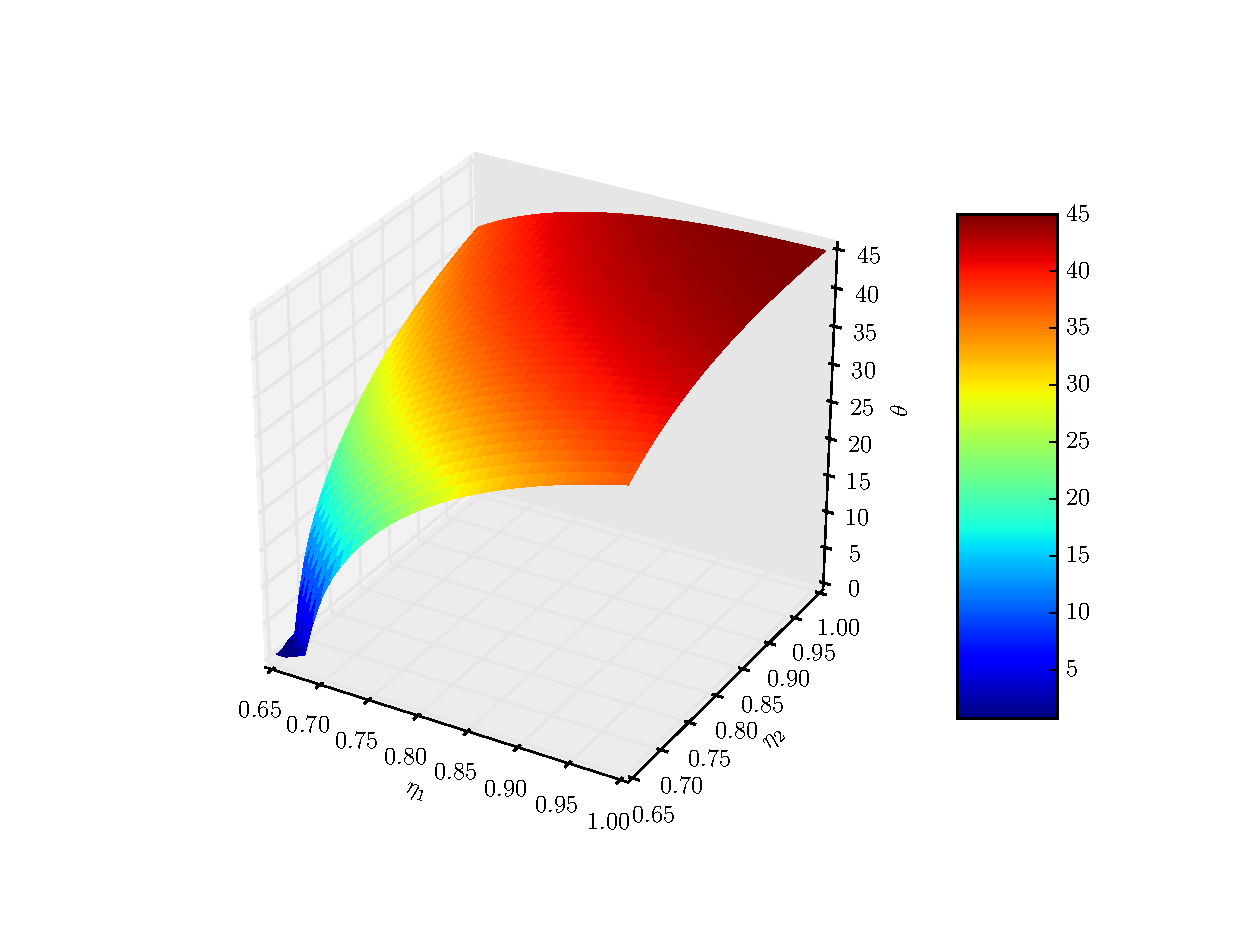
\includegraphics[scale=0.7]{theta3d.eps}
\caption{Оптимизированные значения для $\theta$ для случая различающихся эффективностей детекторов}
\label{fig:theta_opt_3d}
\end{figure}

\begin{figure}[h]
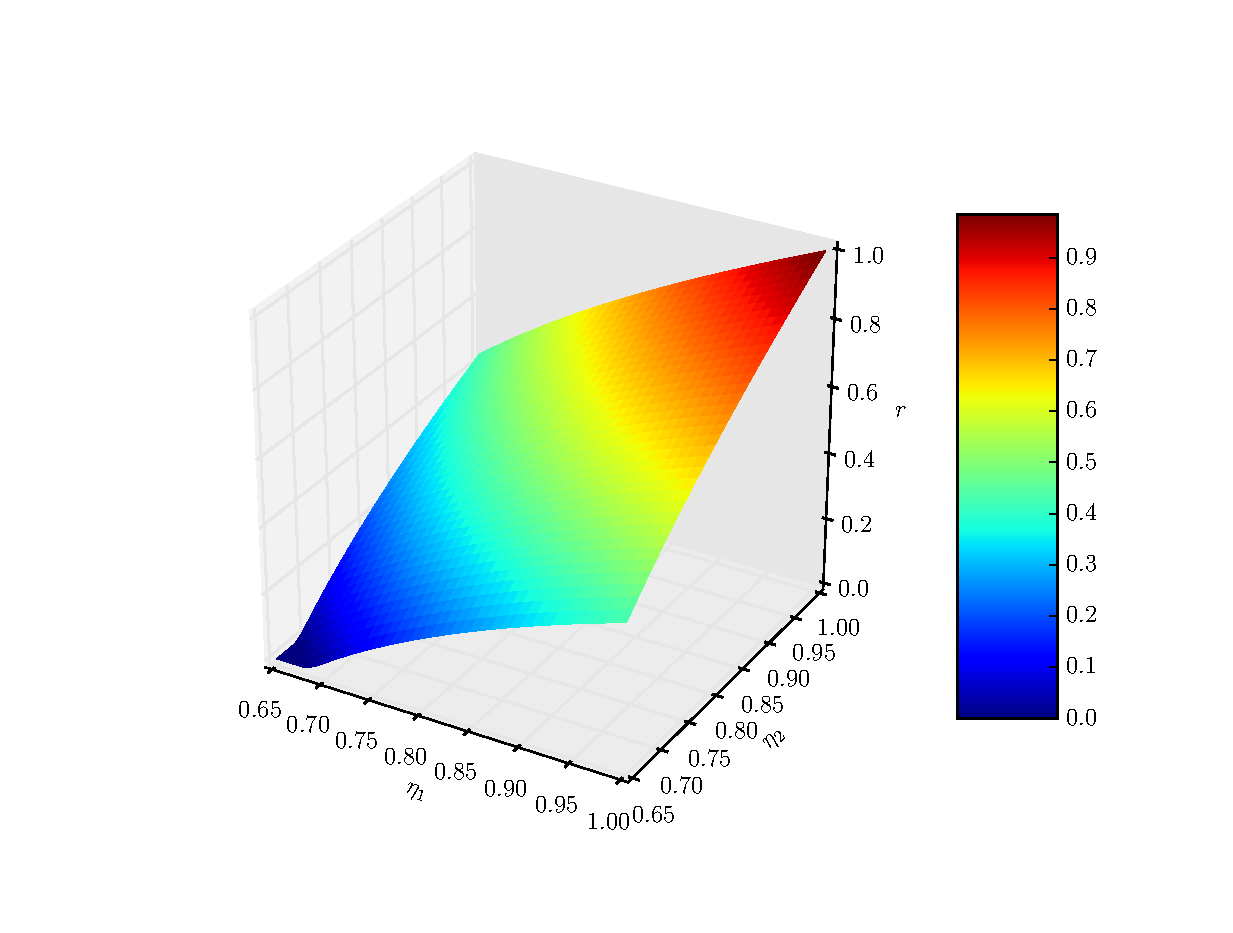
\includegraphics[scale=0.7]{r3d.eps}
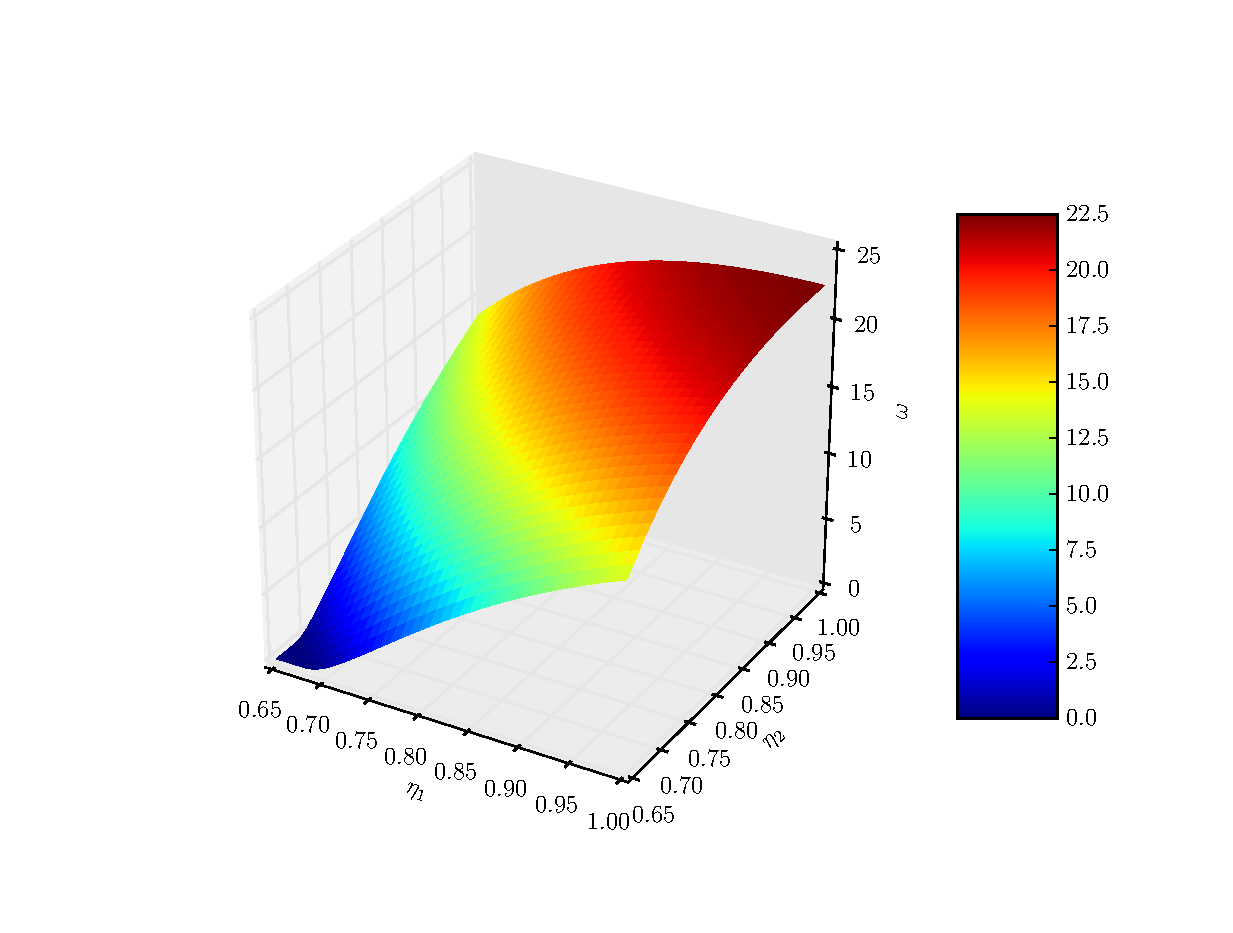
\includegraphics[scale=0.7]{omega3d.eps}
\caption{Оптимизированные значения для $r$ и $\omega$ для случая различающихся эффективностей детекторов}
\label{fig:psi_opt_3d}
\end{figure}

\begin{figure}[t]
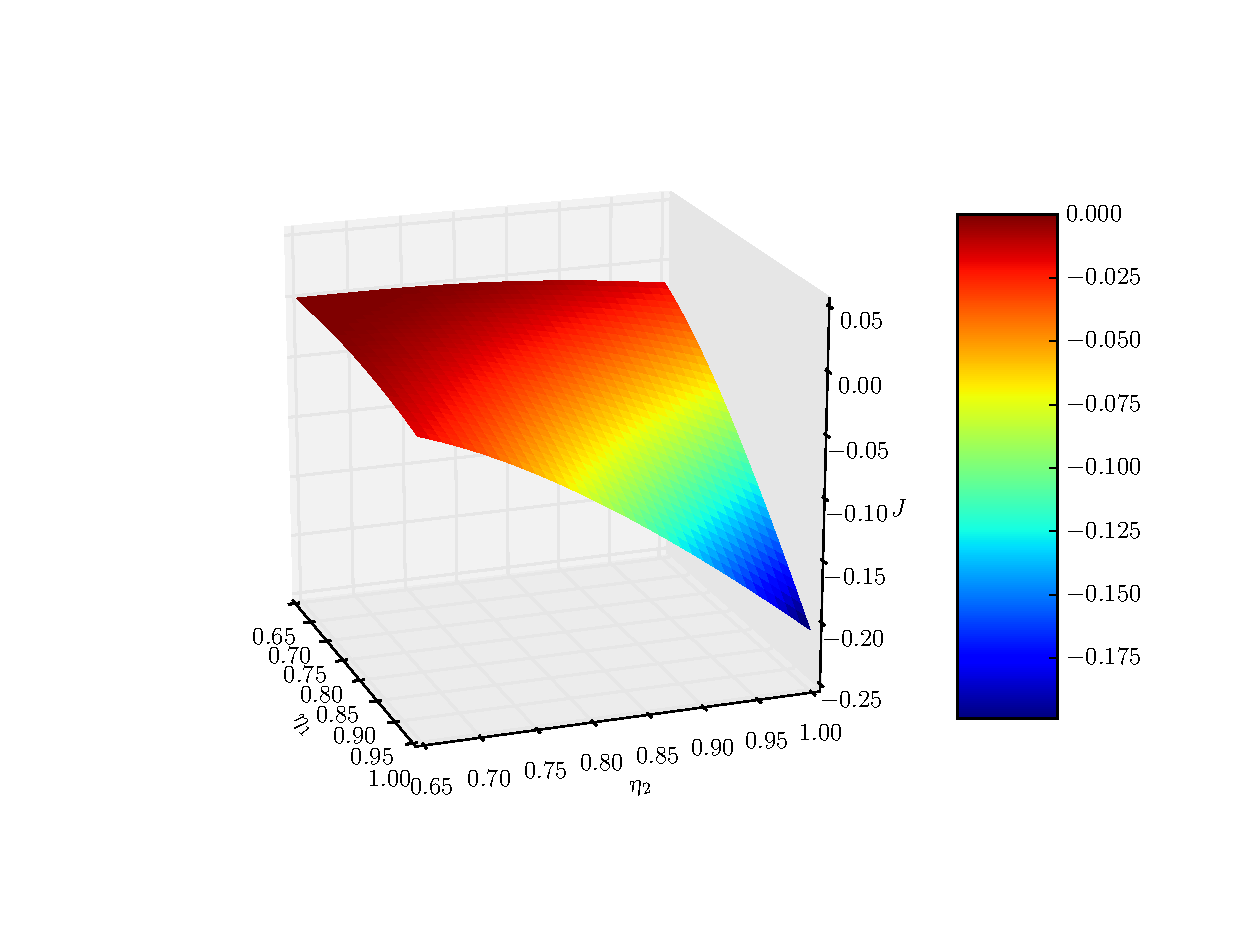
\includegraphics[scale=0.7]{J3d.eps}
\caption{Оптимизированные значения для $J_{\mathcal{B}}/N$ для случая различающихся эффективностей детекторов}
\label{fig:J_opt_3d}
\end{figure}

На рисунках \ref{fig:theta_opt_3d} - \ref{fig:J_opt_3d} изображены значения оптимальных параметров, а также минимизируемой функции для случая различающихся эффективностей.

\begingroup
\small

\begin{longtable}{|c|c|c|c|c|c|c|}
\hline
$\eta_1$ & $\eta_2$ & $r$ & $\omega,^\circ$ & $\theta,^\circ$ & $J_{\mathcal{B}}/N$ & $\zeta$
\\\hline
\endfirsthead

\hline
$\eta_1$ & $\eta_2$ & $r$ & $\omega,^\circ$ & $\theta,^\circ$ & $J_{\mathcal{B}}/N$ & $\zeta$
\\\hline
\endhead


\endfoot

\endlastfoot

\hline
0.65 & 0.65 & 9.73816e-05 & 5.32909e-05 & 0.609422 & 4.13366e-10 & --\\\hline
0.65 & 0.7 & 0.0325726 & 0.4367 & 10.3918 & -5.37452e-06 & 2.68726e-06\\\hline
0.65 & 0.75 & 0.122804 & 2.94407 & 20.3249 & -0.000327839 & 0.00016392\\\hline
0.65 & 0.8 & 0.199412 & 5.64399 & 25.8864 & -0.00152446 & 0.000762231\\\hline
0.65 & 0.85 & 0.266448 & 8.1196 & 29.7694 & -0.00385363 & 0.00192682\\\hline
0.65 & 0.9 & 0.326193 & 10.2951 & 32.6807 & -0.00737942 & 0.00368971\\\hline
0.65 & 0.95 & 0.380046 & 12.1725 & 34.9409 & -0.0120653 & 0.00603265\\\hline
0.65 & 1 & 0.42905 & 13.7822 & 36.7384 & -0.0178271 & 0.00891353\\\hline
0.7 & 0.65 & 0.0325721 & 0.436691 & 10.3917 & -5.37452e-06 & 2.68726e-06\\\hline
0.7 & 0.7 & 0.136389 & 3.40081 & 21.4266 & -0.000453562 & 0.000226781\\\hline
0.7 & 0.75 & 0.223629 & 6.53572 & 27.3754 & -0.00217282 & 0.00108641\\\hline
0.7 & 0.8 & 0.299639 & 9.33741 & 31.4432 & -0.00551773 & 0.00275887\\\hline
0.7 & 0.85 & 0.367155 & 11.7325 & 34.4284 & -0.0105412 & 0.00527059\\\hline
0.7 & 0.9 & 0.427895 & 13.7454 & 36.6985 & -0.0171516 & 0.0085758\\\hline
0.7 & 0.95 & 0.48304 & 15.4224 & 38.4617 & -0.0251977 & 0.0125989\\\hline
0.7 & 1 & 0.533433 & 16.8118 & 39.8493 & -0.034513 & 0.0172565\\\hline
0.75 & 0.65 & 0.122804 & 2.94407 & 20.3249 & -0.000327839 & 0.00016392\\\hline
0.75 & 0.7 & 0.223629 & 6.53572 & 27.3754 & -0.00217282 & 0.00108641\\\hline
0.75 & 0.75 & 0.310518 & 9.73143 & 31.9603 & -0.00615095 & 0.00307547\\\hline
0.75 & 0.8 & 0.387235 & 12.4151 & 35.2194 & -0.0123604 & 0.0061802\\\hline
0.75 & 0.85 & 0.455977 & 14.6188 & 37.6299 & -0.0206635 & 0.0103318\\\hline
0.75 & 0.9 & 0.518149 & 16.4057 & 39.45 & -0.0308332 & 0.0154166\\\hline
0.75 & 0.95 & 0.574864 & 17.8435 & 40.8423 & -0.0426257 & 0.0213128\\\hline
0.75 & 1 & 0.626962 & 18.9919 & 41.9138 & -0.0558135 & 0.0279068\\\hline
0.8 & 0.65 & 0.199412 & 5.64399 & 25.8864 & -0.00152446 & 0.000762231\\\hline
0.8 & 0.7 & 0.299639 & 9.33741 & 31.4432 & -0.00551773 & 0.00275887\\\hline
0.8 & 0.75 & 0.387235 & 12.4151 & 35.2194 & -0.0123604 & 0.0061802\\\hline
0.8 & 0.8 & 0.465228 & 14.8979 & 37.9215 & -0.02191 & 0.010955\\\hline
0.8 & 0.85 & 0.535462 & 16.8648 & 39.9011 & -0.0338613 & 0.0169307\\\hline
0.8 & 0.9 & 0.59933 & 18.4036 & 41.3692 & -0.0478775 & 0.0239387\\\hline
0.8 & 0.95 & 0.657889 & 19.5935 & 42.4623 & -0.063646 & 0.031823\\\hline
0.8 & 1 & 0.712001 & 20.5014 & 43.274 & -0.0808982 & 0.0404491\\\hline
0.85 & 0.65 & 0.266448 & 8.1196 & 29.7694 & -0.00385363 & 0.00192682\\\hline
0.85 & 0.7 & 0.367155 & 11.7325 & 34.4284 & -0.0105412 & 0.00527059\\\hline
0.85 & 0.75 & 0.455977 & 14.6188 & 37.6299 & -0.0206635 & 0.0103318\\\hline
0.85 & 0.8 & 0.535462 & 16.8648 & 39.9011 & -0.0338613 & 0.0169307\\\hline
0.85 & 0.85 & 0.607424 & 18.5808 & 41.5341 & -0.0496902 & 0.0248451\\\hline
0.85 & 0.9 & 0.673214 & 19.8694 & 42.7109 & -0.0677295 & 0.0338647\\\hline
0.85 & 0.95 & 0.733924 & 20.817 & 43.552 & -0.087619 & 0.0438095\\\hline
0.85 & 1 & 0.790464 & 21.4958 & 44.1427 & -0.109064 & 0.0545318\\\hline
0.9 & 0.65 & 0.326193 & 10.2951 & 32.6807 & -0.00737942 & 0.00368971\\\hline
0.9 & 0.7 & 0.427895 & 13.7454 & 36.6985 & -0.0171516 & 0.0085758\\\hline
0.9 & 0.75 & 0.518149 & 16.4057 & 39.45 & -0.0308332 & 0.0154166\\\hline
0.9 & 0.8 & 0.59933 & 18.4036 & 41.3692 & -0.0478775 & 0.0239387\\\hline
0.9 & 0.85 & 0.673214 & 19.8694 & 42.7109 & -0.0677295 & 0.0338647\\\hline
0.9 & 0.9 & 0.741202 & 20.9153 & 43.6381 & -0.0899078 & 0.0449539\\\hline
0.9 & 0.95 & 0.804477 & 21.6349 & 44.2627 & -0.11402 & 0.0570101\\\hline
0.9 & 1 & 0.863896 & 22.1002 & 44.661 & -0.139755 & 0.0698776\\\hline
0.95 & 0.65 & 0.380046 & 12.1725 & 34.9409 & -0.0120653 & 0.00603265\\\hline
0.95 & 0.7 & 0.48304 & 15.4224 & 38.4617 & -0.0251977 & 0.0125989\\\hline
0.95 & 0.75 & 0.574864 & 17.8435 & 40.8423 & -0.0426257 & 0.0213128\\\hline
0.95 & 0.8 & 0.657889 & 19.5935 & 42.4623 & -0.063646 & 0.031823\\\hline
0.95 & 0.85 & 0.733924 & 20.817 & 43.552 & -0.087619 & 0.0438095\\\hline
0.95 & 0.9 & 0.804477 & 21.6349 & 44.2627 & -0.11402 & 0.0570101\\\hline
0.95 & 0.95 & 0.87067 & 22.141 & 44.6958 & -0.142436 & 0.0712182\\\hline
0.95 & 1 & 0.933431 & 22.4101 & 44.924 & -0.172546 & 0.086273\\\hline
1 & 0.65 & 0.42905 & 13.7822 & 36.7384 & -0.0178271 & 0.00891353\\\hline
1 & 0.7 & 0.533433 & 16.8118 & 39.8493 & -0.034513 & 0.0172565\\\hline
1 & 0.75 & 0.626962 & 18.9919 & 41.9138 & -0.0558135 & 0.0279068\\\hline
1 & 0.8 & 0.712001 & 20.5014 & 43.274 & -0.0808982 & 0.0404491\\\hline
1 & 0.85 & 0.790464 & 21.4958 & 44.1427 & -0.109064 & 0.0545318\\\hline
1 & 0.9 & 0.863896 & 22.1002 & 44.661 & -0.139755 & 0.0698776\\\hline
1 & 0.95 & 0.933431 & 22.4101 & 44.924 & -0.172546 & 0.086273\\\hline
1 & 1 & 0.999997 & 22.5 & 45 & -0.207107 & 0.103553\\\hline
\caption{Значения оптимальных параметров для случая различающихся эффективностей}
\label{tab:different_etas}
\end{longtable}

\endgroup

Значения параметров, полученные в ходе оптимизации, а также значения максимально допустимого уровня шума представлены в таблице \ref{tab:different_etas}. Чем выше каждое значение эффективности в отдельности, тем сильнее может быть нарушено неравенство. Минимальные значения эффективностей, при которых нарушение возможно, близки к значению $\eta_1 = \eta_2 = 0.67$, что согласуется с результатами Эберхарда.

%\clearpage

В общем случае для любого состояния $\psi$, минимизирующего величину мат. ожидания, справедливо следующее утверждение.

\begin{theorem}
Квантовое состояние $\psi$, минимизирующее целевую функцию $J$, является собственным вектором матрицы $\mathcal{B}$ и обращает дисперсию в ноль.
\end{theorem}
\begin{proof}
По теореме Куранта-Фишера $\lambda_1 \leq \langle\mathcal{B}\psi, \psi\rangle \leq \lambda_n$, где $\lambda_1, \ldots \lambda_n$ - собственные значения, отсортированные в порядке возрастания. Минимум $J_\mathcal{B} = \langle\mathcal{B}\psi, \psi\rangle = \lambda_1$ достигается, если $\psi = \psi_1$ является собственным вектором. 

Для величины дисперсии в этом случае имеем:
\[\sigma^2 = \langle B^2\rangle - \langle B\rangle^2 = \psi^\dagger B^2 \psi - \lambda_1^2 = \psi^\dagger B \lambda_1  \psi - \lambda_1^2 = 0.
\]
\end{proof}

Это означает, что найденные состояния являются оптимальными не только с точки зрения математического ожидания для количества различных комбинаций измерения поляризации, но и с точки зрения возможного разброса результатов измерений, выраженного через дисперсию.

\section{Оптимизация параметров для модели Цайлингера}
В статье \cite{Zeilinger} рассматривается проверка неравенства Эберхарда применительно к реальному эксперименту. Значения величин $n_{ou}, n_{uo}$ в условиях эксперимента находились по формулам:
\[
n_{ou}(\alpha_1, \beta_2) = S_o^A(\alpha_1) - n_{oo}(\alpha_1, \beta_2) - n_{oe}(\alpha_1, \beta_2),
\]
\[
n_{uo}(\alpha_2, \beta_1) = S_o^B(\beta_1) - n_{oo}(\alpha_2, \beta_1) - n_{eo}(\alpha_2, \beta_1),
\]
где $S_o^A, S_o^B$ - количество срабатываний в обыкновенном луче для первой и второй системы соответственно.

В таком случае неравенство Эберхарда принимает вид:
\begin{equation}
J = -n_{oo}(\alpha_1, \beta_1) + S_o^A(\alpha_1) - n_{oo}(\alpha_1, \beta_2) + S_o^B(\beta_1) - n_{oo}(\alpha_2, \beta_1) + n_{oo}(\alpha_2, \beta_2) \geq 0
\label{eq:Zeilinger_J}
\end{equation}

Рассмотрим оператор плотности в качестве квантового состояния системы:
\[
\rho = \frac{1}{\sqrt{1+r^2}}
\begin{vmatrix}
0 & 0 & 0 & 0\\
0 & 1 & Vr & 0\\
0 & Vr & r^2 & 0\\
0 & 0 & 0 & 0
\end{vmatrix},
\]
где $0 \leq r \leq 1$ и $0 \leq V \leq 1$.
В таком случае предсказания квантовой механики для величин, входящих в состав неравенства, принимают следующий вид:
\begin{eqnarray*}
\tilde{S}_o^A(\alpha_i) = \eta_1 N \Tr[\rho(\hat{P}_A(\alpha_i) \otimes I)]\\
\tilde{S}_o^B(\beta_i) = \eta_1 N \Tr[\rho(I \otimes \hat{P}_B(\beta_i))]\\
\tilde{n}_{oo}(\alpha_i, \beta_i) = \eta_1\eta_2 N \Tr[\rho(\hat{P}_A(\alpha_i) \otimes \hat{P}_B(\beta_i))],
\end{eqnarray*}
где $\hat{P}_A, \hat{P}_B$ - операторы проектирования на направление обыкновенного луча для первой и второй призмы:
\[
\hat{P}(\gamma) = 
\begin{pmatrix}
\cos^2\gamma & \cos\gamma\sin\gamma\\
\cos\gamma\sin\gamma & \sin^2\gamma
\end{pmatrix}.
\]

С учетом ложных срабатываний за время $T$ значения $S_o^A, S_o^B$ принимают вид:
\[
S_o^A(\alpha_i) = \tilde{S}_o^A(\alpha_i) + \zeta T,
\]
\[
S_o^B(\beta_i) = \tilde{S}_o^B(\beta_i) + \zeta T.
\]

Помимо шума модель Цайлингера учитывает несостыковку во времени, когда пары из разных запусков детектируются как сопряженные события. Введем величину временного окна $\tau_c$, в пределах которого должны быть задетектированы сопряженные события. В таком случае значения $n_{oo}(\alpha_i, \beta_i)$ находятся по формулам:
\[
n_{oo}(\alpha_i, \beta_i) = \tilde{n}_{oo}(\alpha_i, \beta_i) + n_{oo}^{acc}(\alpha_i, \beta_i),
\]
\[
n_{oo}^{acc}(\alpha_i, \beta_i) = S_o^A(\alpha_i)S_o^B(\beta_i)\frac{\tau_c}{T}\left(1 - \frac{\tilde{n}_{oo}(\alpha_i, \beta_i)}{S_o^A(\alpha_i)}\right) \left( 1 - \frac{\tilde{n}_{oo}(\alpha_i, \beta_i)}{S_o^B(\beta_i)}\right).
\]

Для данной модели была проведена оптимизация функции $J$ \eqref{eq:Zeilinger_J}, в ходе которой для заданных значений параметров эксперимента($\eta_1, \eta_2, r, V, T, \tau_c, N, \zeta$) были найдены значения углов, минимизирующие целевую функцию.

\begin{table}
\begin{tabular}{|c|c|c|c|c|c|}
\hline 
 & $\alpha_1, ^\circ$ & $\alpha_2, ^\circ$ & $\beta_1, ^\circ$ & $\beta_2, ^\circ$ & $J$ \\ 
\hline 
Результаты из статьи & 85.6 & 118.0 & -5.4 & 25.9 & -120191 \\ 
\hline 
Результаты оптимизации & 85.0 & 115.1 & -4.0 & 27.4 & -126060 \\ 
\hline 
\end{tabular}
\caption{Сравнение оптимальных параметров с параметрами, представленными в статье \cite{Zeilinger}}
\label{tab:Zeilinger_parameters}
\end{table}

Результаты оптимизации представлены в таблице \ref{tab:Zeilinger_parameters}. Согласно полученным значениям, оптимальные величины углов установки призм отличаются от представленных в \cite{Zeilinger} и позволяют нарушить неравенство сильнее.

\section{Нахождение параметров неравенства в случае погрешностей при установке значений углов}
В общем случае квантовый оператор $A$ может быть представлен через спектральную декомпозицию как $A = \int_{-\infty}^{+\infty}\lambda dE_\lambda$. Тогда его мат. ожидание для состояния $\psi$ представимо в виде:
\[
\overline{A}_\psi = \int_{-\infty}^{+\infty}\lambda dp_\psi (\lambda),
\]
где $dp_\psi (\lambda) = d\langle E_\lambda\psi, \psi\rangle$ - распределение вероятностей для соответствующего спектрального разложения и квантового состояния. Поэтому для фиксированного $\psi$ квантовая наблюдаемая может рассматриваться как классическая случайна величина с распределением вероятностей
$p_\psi (O) = \int_O d\langle E_\lambda\psi, \psi\rangle, O\in \mathbb{R}$.

Рассмотрим следующую проблему. Пусть наблюдаемая $A$ зависит от некоторой классической случайной величины $\omega: A = A(\omega)$, что соответствует случаю, когда значения углов положения призм не могут быть выставлены точно в ходе экспериментов. В таком случае спектральное разложение $A(\omega) = \int_{-\infty}^{+\infty}\lambda dE_\lambda(\omega)$ и функция плотности распределения $dp_\psi (\lambda|\omega) = d\langle E_\lambda(\omega)\psi, \psi\rangle$ также зависят от этого случайного параметра. Для любого фиксированного $\omega$ также выполняется условие $\int_{-\infty}^{+\infty}dp_\psi (\lambda|\omega) = 1$.

Пусть случайная величина $\omega$ описывается с помощью вероятностного пространства $(\Omega, \mathcal{F}, P)$, где $\Omega$ - множество элементарных событий, $\mathcal{F}$ - $\sigma$-алгебра событий и $P$ - вероятностная мера. Значение мат. ожидания величины $A(\omega)$ примет вид:
\[
\overline{A}_\psi(\omega) = \int_\Omega\left[\int_{-\infty}^{+\infty}\lambda dp_\psi (\lambda|\omega)\right] dP(\omega) = \int_\Omega\langle A(\omega)\psi, \psi\rangle dP(\omega) = \mathbf{\tilde{E}}[ \langle A(\omega)\psi, \psi\rangle],
\]
где $\mathbf{\tilde{E}}[\cdot]$ - классическое математическое ожидание.

Аналогично получаем выражение для дисперсии $A(\omega)$:
\[
\sigma^2(A) = \mathbf{\tilde{E}}[ \langle A^2(\omega)\psi, \psi\rangle - \langle A(\omega)\psi, \psi\rangle^2].
\]

Будем считать, что реальная величина разности углов $\theta$ в эксперименте равномерно распределена на отрезке вокруг желаемого значения. В этом случае $\theta' = \theta + \xi$, где $\xi$ - случайная величина, равномерно распределенная на отрезке $[-\delta; \delta]$, $\delta > 0$ - параметр разброса. Тогда
\[
J_\mathcal{B} = \frac{1}{2\delta}\int_{-\delta}^\delta \langle \mathcal{B}(r, \omega, \theta + x)\psi, \psi \rangle dx
\] и
\[
\sigma^2 = \frac{1}{2\delta}\int_{-\delta}^\delta (\langle \mathcal{B}^2(r, \omega, \theta + x)\psi, \psi \rangle - \langle \mathcal{B}(r, \omega, \theta + x)\psi, \psi \rangle^2) dx.
\]


Рассмотрим также целевую функцию, которая будет учитывать относительный разброс получаемых значений, выраженный через коэффициент вариации $J / \sigma$. Это позволит получить параметры, при которых при некотором разбросе экспериментальных данных относительная величина будет минимальной.

\begin{figure}[h]
\includegraphics[scale=0.7]{theta_ang.eps}
\caption{Оптимизированные значения для $\theta$ для различных значений $\delta$ в случае $\theta' = \theta + \xi$}
\label{fig:theta_ang}
\end{figure}

\begin{figure}[h]
\includegraphics[scale=0.7]{r_ang.eps}
\includegraphics[scale=0.7]{omega_ang.eps}
\caption{Оптимизированные значения для $r$ и $\omega$ для различных значений $\delta$ в случае $\theta' = \theta + \xi$}
\label{fig:psi_ang}
\end{figure}

\begin{figure}[t]
\includegraphics[scale=0.7]{J_ang.eps}
\caption{Оптимизированные значения для $J_{\mathcal{B}}/N$ для различных значений $\delta$ в случае $\theta' = \theta + \xi$}
\label{fig:J_ang}
\end{figure}


\begingroup
\small

\begin{longtable}{|c|c|c|c|c|c|c|c|c|}
\hline
$\eta$ & $\delta,^\circ$ & $r$ & $\omega,^\circ$ & $\theta,^\circ$ & $J$ & $J_{\delta}$ & $\sigma_{\delta}$ & $K = J_{\delta}/\sigma_{\delta}$
\endfirsthead

\hline
$\eta$ & $\delta,^\circ$ & $r$ & $\omega,^\circ$ & $\theta,^\circ$ & $J$ & $J_{\delta}$ & $\sigma_{\delta}$ & $K = J_{\delta}/\sigma_{\delta}$\\
\hline
\endhead

\hline
\endfoot

\endlastfoot

\hline
\multirow{3}{*}{0.7} & \multirow{3}{*}{0.25} & 0.13639 & 3.4008 & 21.427 & -0.00045356 & -0.00045189 & 0.00087956 & -0.51377\\\cline{3-9}
 &  & 0.13629 & 3.3972 & 21.418 & -0.00045356 & -0.00045189 & 0.00087922 & -0.51397\\\cline{3-9}
 &  & 0.12395 & 2.9245 & 20.237 & -0.00044085 & -0.00043936 & 0.00083444 & -0.52653\\\hline
\multirow{3}{*}{0.7} & \multirow{3}{*}{0.5} & 0.13639 & 3.4008 & 21.427 & -0.00045356 & -0.00044688 & 0.0017591 & -0.25404\\\cline{3-9}
 &  & 0.1361 & 3.3903 & 21.397 & -0.00045355 & -0.00044689 & 0.0017569 & -0.25437\\\cline{3-9}
 &  & 0.12378 & 2.9192 & 20.221 & -0.00044051 & -0.00043455 & 0.0016676 & -0.26059\\\hline
\multirow{3}{*}{0.7} & \multirow{3}{*}{0.75} & 0.13639 & 3.4008 & 21.427 & -0.00045356 & -0.00043854 & 0.0026387 & -0.1662\\\cline{3-9}
 &  & 0.13566 & 3.3739 & 21.357 & -0.00045351 & -0.00043858 & 0.0026307 & -0.16672\\\cline{3-9}
 &  & 0.1235 & 2.91 & 20.193 & -0.00043993 & -0.00042657 & 0.0024981 & -0.17076\\\hline
\multirow{3}{*}{0.7} & \multirow{3}{*}{1.0} & 0.13639 & 3.4008 & 21.427 & -0.00045356 & -0.00042685 & 0.0035182 & -0.12132\\\cline{3-9}
 &  & 0.13513 & 3.3554 & 21.305 & -0.00045341 & -0.000427 & 0.0034994 & -0.12202\\\cline{3-9}
 &  & 0.12306 & 2.8955 & 20.149 & -0.000439 & -0.00041536 & 0.0033239 & -0.12496\\\hline
\multirow{3}{*}{0.75} & \multirow{3}{*}{0.25} & 0.31052 & 9.7314 & 31.96 & -0.0061509 & -0.0061468 & 0.0014539 & -4.2279\\\cline{3-9}
 &  & 0.31047 & 9.729 & 31.956 & -0.0061509 & -0.0061468 & 0.0014537 & -4.2284\\\cline{3-9}
 &  & 0.28314 & 8.2348 & 29.774 & -0.0059469 & -0.0059433 & 0.0013654 & -4.3528\\\hline
\multirow{3}{*}{0.75} & \multirow{3}{*}{0.5} & 0.31052 & 9.7314 & 31.96 & -0.0061509 & -0.0061346 & 0.0029077 & -2.1098\\\cline{3-9}
 &  & 0.31037 & 9.7245 & 31.95 & -0.0061509 & -0.0061346 & 0.0029068 & -2.1104\\\cline{3-9}
 &  & 0.28301 & 8.2297 & 29.765 & -0.0059453 & -0.0059309 & 0.00273 & -2.1725\\\hline
\multirow{3}{*}{0.75} & \multirow{3}{*}{0.75} & 0.31052 & 9.7314 & 31.96 & -0.0061509 & -0.0061141 & 0.0043614 & -1.4019\\\cline{3-9}
 &  & 0.31024 & 9.7187 & 31.939 & -0.0061509 & -0.0061141 & 0.0043587 & -1.4027\\\cline{3-9}
 &  & 0.28288 & 8.2252 & 29.756 & -0.0059437 & -0.0059113 & 0.0040937 & -1.444\\\hline
\multirow{3}{*}{0.75} & \multirow{3}{*}{1.0} & 0.31052 & 9.7314 & 31.96 & -0.0061509 & -0.0060854 & 0.0058149 & -1.0465\\\cline{3-9}
 &  & 0.30998 & 9.7066 & 31.92 & -0.0061509 & -0.0060854 & 0.005808 & -1.0478\\\cline{3-9}
 &  & 0.28269 & 8.219 & 29.743 & -0.0059414 & -0.0058839 & 0.0054558 & -1.0785\\\hline
\multirow{3}{*}{0.8} & \multirow{3}{*}{0.25} & 0.46523 & 14.898 & 37.921 & -0.02191 & -0.021904 & 0.0019372 & -11.307\\\cline{3-9}
 &  & 0.46523 & 14.898 & 37.921 & -0.02191 & -0.021904 & 0.0019372 & -11.307\\\cline{3-9}
 &  & 0.42475 & 12.175 & 34.602 & -0.020989 & -0.020984 & 0.0017892 & -11.728\\\hline
\multirow{3}{*}{0.8} & \multirow{3}{*}{0.5} & 0.46523 & 14.898 & 37.921 & -0.02191 & -0.021884 & 0.0038743 & -5.6485\\\cline{3-9}
 &  & 0.46509 & 14.893 & 37.915 & -0.02191 & -0.021884 & 0.0038737 & -5.6495\\\cline{3-9}
 &  & 0.42467 & 12.172 & 34.597 & -0.020987 & -0.020964 & 0.0035779 & -5.8594\\\hline
\multirow{3}{*}{0.8} & \multirow{3}{*}{0.75} & 0.46523 & 14.898 & 37.921 & -0.02191 & -0.021852 & 0.0058112 & -3.7604\\\cline{3-9}
 &  & 0.46514 & 14.89 & 37.91 & -0.02191 & -0.021852 & 0.0058097 & -3.7614\\\cline{3-9}
 &  & 0.4246 & 12.171 & 34.594 & -0.020985 & -0.020935 & 0.0053661 & -3.9014\\\hline
\multirow{3}{*}{0.8} & \multirow{3}{*}{1.0} & 0.46523 & 14.898 & 37.921 & -0.02191 & -0.021808 & 0.0077478 & -2.8147\\\cline{3-9}
 &  & 0.46492 & 14.885 & 37.901 & -0.02191 & -0.021808 & 0.0077438 & -2.8162\\\cline{3-9}
 &  & 0.42446 & 12.167 & 34.587 & -0.020981 & -0.020893 & 0.0071529 & -2.9209\\\hline
\multirow{3}{*}{0.85} & \multirow{3}{*}{0.25} & 0.60742 & 18.581 & 41.534 & -0.04969 & -0.049682 & 0.0023836 & -20.843\\\cline{3-9}
 &  & 0.60742 & 18.581 & 41.534 & -0.04969 & -0.049682 & 0.0023836 & -20.843\\\cline{3-9}
 &  & 0.55773 & 14.454 & 36.889 & -0.047039 & -0.047032 & 0.0021555 & -21.82\\\hline
\multirow{3}{*}{0.85} & \multirow{3}{*}{0.5} & 0.60742 & 18.581 & 41.534 & -0.04969 & -0.049656 & 0.0047671 & -10.417\\\cline{3-9}
 &  & 0.60742 & 18.581 & 41.532 & -0.04969 & -0.049656 & 0.0047669 & -10.417\\\cline{3-9}
 &  & 0.55773 & 14.456 & 36.89 & -0.047041 & -0.047012 & 0.0043109 & -10.905\\\hline
\multirow{3}{*}{0.85} & \multirow{3}{*}{0.75} & 0.60742 & 18.581 & 41.534 & -0.04969 & -0.049614 & 0.0071502 & -6.9388\\\cline{3-9}
 &  & 0.60728 & 18.572 & 41.523 & -0.04969 & -0.049614 & 0.0071485 & -6.9405\\\cline{3-9}
 &  & 0.55763 & 14.452 & 36.884 & -0.047034 & -0.046969 & 0.0064651 & -7.2651\\\hline
\multirow{3}{*}{0.85} & \multirow{3}{*}{1.0} & 0.60742 & 18.581 & 41.534 & -0.04969 & -0.049554 & 0.0095329 & -5.1983\\\cline{3-9}
 &  & 0.60719 & 18.568 & 41.515 & -0.04969 & -0.049554 & 0.0095291 & -5.2003\\\cline{3-9}
 &  & 0.55754 & 14.452 & 36.882 & -0.047031 & -0.046916 & 0.0086189 & -5.4434\\\hline
\multirow{3}{*}{0.9} & \multirow{3}{*}{0.25} & 0.7412 & 20.915 & 43.638 & -0.089908 & -0.089897 & 0.0028018 & -32.086\\\cline{3-9}
 &  & 0.7412 & 20.915 & 43.638 & -0.089908 & -0.089897 & 0.0028018 & -32.086\\\cline{3-9}
 &  & 0.68917 & 15.162 & 37.368 & -0.083711 & -0.083703 & 0.0024619 & -34\\\hline
\multirow{3}{*}{0.9} & \multirow{3}{*}{0.5} & 0.7412 & 20.915 & 43.638 & -0.089908 & -0.089866 & 0.0056033 & -16.038\\\cline{3-9}
 &  & 0.74119 & 20.912 & 43.633 & -0.089908 & -0.089866 & 0.0056028 & -16.039\\\cline{3-9}
 &  & 0.68916 & 15.163 & 37.368 & -0.083712 & -0.083678 & 0.0049236 & -16.995\\\hline
\multirow{3}{*}{0.9} & \multirow{3}{*}{0.75} & 0.7412 & 20.915 & 43.638 & -0.089908 & -0.089815 & 0.0084045 & -10.686\\\cline{3-9}
 &  & 0.74113 & 20.912 & 43.633 & -0.089908 & -0.089815 & 0.0084036 & -10.688\\\cline{3-9}
 &  & 0.6891 & 15.162 & 37.366 & -0.083708 & -0.083632 & 0.0073846 & -11.325\\\hline
\multirow{3}{*}{0.9} & \multirow{3}{*}{1.0} & 0.7412 & 20.915 & 43.638 & -0.089908 & -0.089742 & 0.011205 & -8.009\\\cline{3-9}
 &  & 0.74109 & 20.905 & 43.626 & -0.089908 & -0.089742 & 0.011202 & -8.011\\\cline{3-9}
 &  & 0.68901 & 15.16 & 37.361 & -0.083698 & -0.083563 & 0.0098441 & -8.4886\\\hline
\multirow{3}{*}{0.95} & \multirow{3}{*}{0.25} & 0.87067 & 22.141 & 44.696 & -0.14244 & -0.14242 & 0.0031944 & -44.586\\\cline{3-9}
 &  & 0.87067 & 22.141 & 44.696 & -0.14244 & -0.14242 & 0.0031944 & -44.586\\\cline{3-9}
 &  & 0.82898 & 14.374 & 36.245 & -0.12911 & -0.1291 & 0.0026843 & -48.093\\\hline
\multirow{3}{*}{0.95} & \multirow{3}{*}{0.5} & 0.87067 & 22.141 & 44.696 & -0.14244 & -0.14239 & 0.0063885 & -22.288\\\cline{3-9}
 &  & 0.87064 & 22.138 & 44.694 & -0.14244 & -0.14239 & 0.0063883 & -22.289\\\cline{3-9}
 &  & 0.82895 & 14.372 & 36.242 & -0.1291 & -0.12906 & 0.005368 & -24.042\\\hline
\multirow{3}{*}{0.95} & \multirow{3}{*}{0.75} & 0.87067 & 22.141 & 44.696 & -0.14244 & -0.14233 & 0.0095822 & -14.853\\\cline{3-9}
 &  & 0.87064 & 22.133 & 44.687 & -0.14244 & -0.14233 & 0.0095806 & -14.856\\\cline{3-9}
 &  & 0.8289 & 14.371 & 36.239 & -0.12909 & -0.129 & 0.0080509 & -16.023\\\hline
\multirow{3}{*}{0.95} & \multirow{3}{*}{1.0} & 0.87067 & 22.141 & 44.696 & -0.14244 & -0.14224 & 0.012775 & -11.134\\\cline{3-9}
 &  & 0.8706 & 22.13 & 44.682 & -0.14244 & -0.14224 & 0.012772 & -11.137\\\cline{3-9}
 &  & 0.82884 & 14.369 & 36.233 & -0.12907 & -0.12892 & 0.010732 & -12.013\\\hline
\multirow{3}{*}{1.0} & \multirow{3}{*}{0.25} & 1 & 22.5 & 45 & -0.20711 & -0.20709 & 0.0035626 & -58.13\\\cline{3-9}
 &  & 1 & 22.5 & 45 & -0.20711 & -0.20709 & 0.0035626 & -58.13\\\cline{3-9}
 &  & 1 & 11.859 & 33.084 & -0.17763 & -0.17762 & 0.0027502 & -64.585\\\hline
\multirow{3}{*}{1.0} & \multirow{3}{*}{0.5} & 1 & 22.5 & 45 & -0.20711 & -0.20705 & 0.0071249 & -29.06\\\cline{3-9}
 &  & 1 & 22.497 & 44.995 & -0.20711 & -0.20705 & 0.0071244 & -29.063\\\cline{3-9}
 &  & 1 & 11.86 & 33.084 & -0.17763 & -0.1776 & 0.0055003 & -32.289\\\hline
\multirow{3}{*}{1.0} & \multirow{3}{*}{0.75} & 1 & 22.5 & 45 & -0.20711 & -0.20699 & 0.010687 & -19.368\\\cline{3-9}
 &  & 0.99997 & 22.493 & 44.992 & -0.20711 & -0.20699 & 0.010685 & -19.371\\\cline{3-9}
 &  & 1 & 11.86 & 33.081 & -0.17762 & -0.17754 & 0.0082493 & -21.522\\\hline
\multirow{3}{*}{1.0} & \multirow{3}{*}{1.0} & 1 & 22.5 & 45 & -0.20711 & -0.20689 & 0.014248 & -14.521\\\cline{3-9}
 &  & 1 & 22.491 & 44.987 & -0.20711 & -0.20689 & 0.014244 & -14.524\\\cline{3-9}
 &  & 0.99999 & 11.855 & 33.072 & -0.17758 & -0.17744 & 0.010995 & -16.137\\\hline
 \caption{Сравнение значений параметров при различных способах минимизации: 1 строка - минимизация $J_\mathcal{B}$ без учета $\delta$, 2 строка - минимизация $J(\delta)$, 3 строка - минимизация $K = J(\delta) / \sigma(\delta)$}
 \label{tab:one_delta}
\end{longtable}
\endgroup

Сравнение результатов для различных значений $\delta$ представлены на графиках \ref{fig:theta_ang} - \ref{fig:J_ang}, а также в таблице \ref{tab:one_delta}. Строки в таблице \ref{tab:one_delta} для заданных значений $\eta$ и $\delta$ сгруппированы по три: первая строка - минимизация $J_\mathcal{B}$ без учета $\delta$, вторая строка - минимизация $J(\delta)$, третья строка - минимизация $K = J(\delta) / \sigma(\delta)$. 

Так как реальные значения эффективностей - около $\eta = 0.85$, то из второго графика видно, что значения мат. ожидания не сильно отличаются от случая нулевой эффективности. Кроме того, для различных значений $\delta$ в пределах одного градуса графики почти совпадают.

Усложним модель разброса - будем рассматривать погрешность каждого угла в отдельности. Будем считать, что реальная величина каждого угла в эксперименте равномерно распределена на отрезке вокруг желаемого значения. В этом случае значения мат. ожидания и дисперсии принимают следующий вид:
\[
J_\mathcal{B} = \frac{1}{16\delta^4}\int\int\int\int_{-\delta}^\delta \langle \mathcal{B}(x_1, x_2, x_3, x_4)\psi, \psi \rangle dx_1dx_2dx_3dx_4,
\] 
\[
\sigma^2 = \frac{1}{16\delta^4}\int\int\int\int_{-\delta}^\delta (\langle \mathcal{B}^2\psi, \psi \rangle - \langle \mathcal{B}\psi, \psi \rangle^2) dx_1dx_2dx_3dx_4.
\]

\begin{figure}[h]
\includegraphics[scale=0.7]{theta_4ang.eps}
\caption{Оптимизированные значения для $\theta$ для различных значений углов}
\label{fig:theta_4ang}
\end{figure}

\begin{figure}[h]
\includegraphics[scale=0.7]{r_4ang.eps}
\includegraphics[scale=0.7]{omega_4ang.eps}
\caption{Оптимизированные значения для $r$ и $\omega$ для различных значений углов}
\label{fig:psi_4ang}
\end{figure}

\begin{figure}[t]
\includegraphics[scale=0.7]{K_4ang.eps}
\caption{Оптимизированные значения для $J_{\mathcal{B}}/N$ для различных значений углов}
\label{fig:J_4ang}
\end{figure}

\begin{table}
\small
\begin{tabular}{|c|c|c|c|c|c|c|c|c|}
\hline
$\eta$ & $\delta,^\circ$ & $r$ & $\omega,^\circ$ & $\theta,^\circ$ & $J$ & $J_{\delta}$ & $\sigma_{\delta}$ & $K = J_{\delta}/\sigma_{\delta}$
\\\hline
\multirow{3}{*}{0.7} & \multirow{3}{*}{0.25} & 0.136389 & 3.40081 & 21.4266 & -0.000453562 & -0.000444565 & 0.00241554 & -0.184044\\\cline{3-9}
 &  & 0.136389 & 3.40081 & 21.4266 & -0.000453562 & -0.000444565 & 0.00241554 & -0.184044\\\cline{3-9}
 &  & 0.137124 & 3.42997 & 21.496 & -0.000453514 & -0.000444515 & 0.00241503 & -0.184062\\\hline
 \multirow{3}{*}{0.75} & \multirow{3}{*}{0.25} & 0.310518 & 9.73143 & 31.9603 & -0.00615095 & -0.00614082 & 0.00248895 & -2.46724\\\cline{3-9}
 &  & 0.310518 & 9.73143 & 31.9603 & -0.00615095 & -0.00614082 & 0.00248895 & -2.46724\\\cline{3-9}
 &  & 0.313658 & 9.91344 & 32.2158 & -0.00614786 & -0.00613773 & 0.00248642 & -2.4685\\\hline
\multirow{3}{*}{0.8} & \multirow{3}{*}{0.25} & 0.465228 & 14.8979 & 37.9215 & -0.02191 & -0.0218985 & 0.002596 & -8.43546\\\cline{3-9}
 &  & 0.465228 & 14.8979 & 37.9215 & -0.02191 & -0.0218985 & 0.002596 & -8.43546\\\cline{3-9}
 &  & 0.469841 & 15.2419 & 38.3231 & -0.0218953 & -0.0218838 & 0.00259252 & -8.44116\\\hline
\multirow{3}{*}{0.85} & \multirow{3}{*}{0.25} & 0.607424 & 18.5808 & 41.5341 & -0.0496902 & -0.0496772 & 0.00275221 & -18.0499\\\cline{3-9}
 &  & 0.607424 & 18.5808 & 41.5341 & -0.0496902 & -0.0496772 & 0.00275221 & -18.0499\\\cline{3-9}
 &  & 0.61123 & 18.9498 & 41.9292 & -0.0496699 & -0.0496569 & 0.00274992 & -18.0576\\\hline
\multirow{3}{*}{0.9} & \multirow{3}{*}{0.25} & 0.741202 & 20.9153 & 43.6381 & -0.0899078 & -0.0898932 & 0.00296469 & -30.3213\\\cline{3-9}
 &  & 0.741202 & 20.9153 & 43.6381 & -0.0899078 & -0.0898932 & 0.00296469 & -30.3213\\\cline{3-9}
 &  & 0.743038 & 21.167 & 43.8961 & -0.0898969 & -0.0898824 & 0.00296395 & -30.3252\\\hline
\multirow{3}{*}{0.95} & \multirow{3}{*}{0.25} & 0.87067 & 22.141 & 44.6958 & -0.142436 & -0.14242 & 0.00323493 & -44.0258\\\cline{3-9}
 &  & 0.87067 & 22.141 & 44.6958 & -0.142436 & -0.14242 & 0.00323493 & -44.0258\\\cline{3-9}
 &  & 0.871004 & 22.2272 & 44.7823 & -0.142435 & -0.142419 & 0.00323486 & -44.0263\\\hline
\multirow{3}{*}{1.0} & \multirow{3}{*}{0.25} & 0.999997 & 22.5 & 45 & -0.207107 & -0.207089 & 0.0035626 & -58.1286\\\cline{3-9}
 &  & 0.999997 & 22.5 & 45 & -0.207107 & -0.207089 & 0.0035626 & -58.1286\\\cline{3-9}
 &  & 0.999999 & 22.4981 & 44.998 & -0.207107 & -0.207089 & 0.0035626 & -58.1286\\\hline
 \end{tabular}
\caption{Значения оптимизированных параметров для погрешности в четырех углах в отдельности для случай $\delta = 0.25^\circ$}
\label{tab:different_deltas}
\end{table}


Результаты проведенной оптимизации представлены на рисунках \ref{fig:theta_4ang} - \ref{fig:J_4ang} и в таблице \ref{tab:different_deltas}, строки которой также сгруппированы по три. Из графиков видно, что добавление разброса почти не изменяет оптимальные параметры. А это означает, что можно сделать предположение, что контроль за величиной углов детекторов можно уменьшить. 

\conclusion
В ходе выполнения работы была рассмотрена модель Эберхарда, описывающая предсказания квантовой механики для случая одинаковых эффективностей детекторов. Для этой модели была проведена оптимизация параметров, результаты которой согласуются с аналогичными результатами из рассматриваемой статьи. Аналогичная процедура была проведена для случая различных эффективностей. Заметим, что в работе Эберхарда был изучен лишь случай детекторов, имеющих равную эффективность. Однако в реальных экспериментах эффективности детекторов могут существенно отличаться.

Кроме того, было высказано предположение, что для оценки степени нарушения необходимо использовать целевую функцию, учитывающую величину возможного разброса экспериментальных данных, выраженную через коэффициент вариации $\sigma_J / J$. Было показано, что в модели, описанной Эберхардом, минимальное значение математического ожидания достигается для $\psi$, равного собственному вектору матрицы $\mathcal{B}$, и дисперсия в этом случае равна нулю.

Однако, в случае, если в модель добавляется погрешность установки поляризационных призм, выраженная через погрешности углов, то эта целевая функция позволяет найти такие параметры, при которых неравенство будет нарушаться даже с учетом возможных погрешностей. Полученные параметры отличаются от результатов Эберхарда. Недавно (май 2014) проф. Хренников  обсуждал эти результаты с сотрудниками лаборатории квантовой оптики и информации Венского университета. Результаты моделирования вызвали интерес у экспериментаторов, так как позволяют ослабить контроль над точностью ориентации осей поляризационных призм.

Кроме того, была рассмотрена реализация тестирования неравенства Эберхарда из статьи \cite{Zeilinger}. Для параметров, указанных там, при заданных значениях эффективностей была также проведена оптимизация. При подстановке полученных значений в модели Цайлингера наблюдается более сильное нарушение неравенства, чем указанное в статье. Эти результаты также обсуждались с экспериментаторами из Вены. Оказалось, что они активно работают над этой проблемой: объяснения расхождения теоретических и экспериментальных значений, а также расхождении между значениями, предсказываемыми различными моделями.

Полученные результаты позволяют ожидать, что при проведении экспериментов с найденными значениями будут получены результаты, нарушающие неравенство Эберхарда даже с учетом различных эффективностей детекторов и погрешностями в установке углов.

\bibliography{literature_rus}
\bibliographystyle{ugost2008}
%\bibliographystyle{gost705}
\end{document}
